\documentclass[12pt]{amsart}
%\usepackage{tweaklist}
\usepackage{cancel}
\usepackage{xspace}
\usepackage[utf8]{inputenc}
\usepackage{graphicx}
\usepackage{multicol}
\usepackage{subfig}
\usepackage{amsmath}
\usepackage{amssymb}
\usepackage[a4paper,width=160mm,top=18mm,bottom=21mm,includeheadfoot]{geometry}
\usepackage{booktabs}
\usepackage{array}
\usepackage{verbatim}
\usepackage{caption}
% \usepackage{natbib}

\usepackage{float}
\usepackage{pdflscape}
\usepackage{mathtools}
\usepackage[usenames,dvipsnames]{xcolor}
\usepackage{afterpage}
\usepackage{tikz}
\usepackage[hyperfootnotes=false, bookmarks=true, unicode=true, pdftitle={Ethereum Yellow Paper: a formal specification of Ethereum, a programmable blockchain}, pdfauthor={Dr. Gavin Wood},pdfkeywords={Ethereum, Yellow Paper, blockchain, virtual machine, cryptography, decentralised, singleton, transaction, generalised},pdfborder={0 0 0.5 [1 3]}]{hyperref}
%,pagebackref=true

\usepackage{tabu} %requires array.
\def\els@aparagraph[#1]#2{\elsparagraph[#1]{#2}}
\def\els@bparagraph#1{\elsparagraph*{#1}}
\newcommand\eatpunct[1]{}
%This should be the last package before \input{Version.tex}
\PassOptionsToPackage{hyphens}{url}\usepackage{hyperref}
% "hyperref loads the url package internally. Use \PassOptionsToPackage{hyphens}{url}\usepackage{hyperref} to pass the option to the url package when it is loaded by hyperref. This avoids any package option clashes." Source: <https://tex.stackexchange.com/questions/3033/forcing-linebreaks-in-url/3034#comment44478_3034>.
% Note also this: "If the \PassOptionsToPackage{hyphens}{url} approach does not work, maybe it's "because you're trying to load the url package with a specific option, but it's being loaded by one of your packages before that with a different set of options. Try loading the url package earlier than the package that requires it. If it's loaded by the document class, try using \RequirePackage[hyphens]{url} before the document class." Source: <https://tex.stackexchange.com/questions/3033/forcing-linebreaks-in-url/3034#comment555944_3034>.
% For more information on using the hyperref package, refer to e.g. https://en.wikibooks.org/w/index.php?title=LaTeX/Hyperlinks&stable=0#Hyperlink_and_Hypertarget.

\makeatletter
 \newcommand{\linkdest}[1]{\Hy@raisedlink{\hypertarget{#1}{}}}
\makeatother
\usepackage{seqsplit}

% For formatting
%\usepackage{underscore}
%\usepackage{lipsum} % to generate filler text for testing of document rendering
\usepackage[english]{babel}
\usepackage[autostyle]{csquotes}
\MakeOuterQuote{"}

\usepackage[final]{microtype} % https://tex.stackexchange.com/questions/75140/is-it-possible-to-make-latex-mark-overfull-boxes-in-the-output#comment382776_75142
\usepackage{lastpage}
\usepackage{footnote}
\usepackage{caption}
\definecolor{Orange}{rgb}{0.241,0.349,0.090}
% \usepackage{bbding}
\usepackage{shortvrb}
%% \usepackage{draftwatermark}
%% \SetWatermarkText{Esborrany}
%% \SetWatermarkScale{0.5}
%% \usepackage{tocloft}
% \usepackage{hyperref}
% \usepackage{bookmark}
\usepackage[titletoc]{appendix}


% \input{Version.tex}
% Default rendering options
\definecolor{pagecolor}{rgb}{1,0.98,0.9}
\def\YellowPaperVersionNumber{unknown revision}
\IfFileExists{Options.tex}{\input{Options.tex}}

\newcommand{\hcancel}[1]{%
    \tikz[baseline=(tocancel.base)]{
        \node[inner sep=0pt,outer sep=0pt] (tocancel) {#1};
        \draw[black] (tocancel.south west) -- (tocancel.north east);
    }%
}%


\DeclarePairedDelimiter{\ceil}{\lceil}{\rceil}
\newcommand*\eg{e.g.\@\xspace}
\newcommand*\Eg{e.g.\@\xspace}
\newcommand*\ie{i.e.\@\xspace}
%\renewcommand{\itemhook}{\setlength{\topsep}{0pt}  \setlength{\itemsep}{0pt}\setlength{\leftmargin}{15pt}}


\title{Wireless service accounting based on Ethereum state channels
- Master Thesis}

\author{
  A. Egio,
  L. González, A. Pardo, T. Romero
}


\begin{document}

\pagecolor{pagecolor}


\begin{abstract}
%  \begin{center}
    This document contains authors' ``\textit{Blockchain
      technologies master}''\footnote{UPC School
      of Professional \& Executive Development}
    thesis. The project described in the document
    consists on a technological proof
    of concept of an internet access service consumption
    using a state channel smart contract as
    mean of payment. After a brief
    introduction, there's a first motivation of
    the use case included;
    in the following sections
    there's a detailed explanation of
    the architecture, implementation and
    security considerations;
    after that it is described a more
    general approach about using blockchain technologies
    and state channels to provide
    mechanisms to reduce advanced wireless
    (i. e. 5G) services market friction between neutral host
    providers, virtual operators and operators
    purchasing licenses of spectrum bands to nations' governments;
    ideally achieving an unprecedented transparency guarantee to consumers and
    a fully GDPR compliant
    schema relying on a self-sovereign identity system.

%  \end{center}
\end{abstract}

\maketitle

\tableofcontents

\newpage

\vspace*{5cm}

% \begin{center}
\Huge{\textbf{DISCLAIMER}}
\vspace{1cm}


\Large
All software described and linked in this document is open source
under the MIT license; so anyone can freely use it and make
modifications to the source code to fulfill their use
cases. But if you do so, please take into account that the software
at the time of this writing is merely
a proof of concept and is not properly audited; although
authors tried to follow best practices regarding smart contract,
front-end and back-end design and implementation there are still
some trade-offs and recognizable security issues
described in this document's
security considerations section. Please take this into account
when using and/or modifying this software and be conscious
that authors do not provide any guarantee in case of
security issues, economical loses or regulation infringement.
% \end{center}

\vspace{1cm}

\newpage

\vspace*{5cm}
\normalsize
\begin{verbatim}
MIT License

Copyright (c) 2019 ethereum-internet-access

Permission is hereby granted, free of charge, to any person obtaining a copy
of this software and associated documentation files (the "Software"), to deal
in the Software without restriction, including without limitation the rights
to use, copy, modify, merge, publish, distribute, sublicense, and/or sell
copies of the Software, and to permit persons to whom the Software is
furnished to do so, subject to the following conditions:

The above copyright notice and this permission notice shall be included in all
copies or substantial portions of the Software.

THE SOFTWARE IS PROVIDED "AS IS", WITHOUT WARRANTY OF ANY KIND, EXPRESS OR
IMPLIED, INCLUDING BUT NOT LIMITED TO THE WARRANTIES OF MERCHANTABILITY,
FITNESS FOR A PARTICULAR PURPOSE AND NONINFRINGEMENT. IN NO EVENT SHALL THE
AUTHORS OR COPYRIGHT HOLDERS BE LIABLE FOR ANY CLAIM, DAMAGES OR OTHER
LIABILITY, WHETHER IN AN ACTION OF CONTRACT, TORT OR OTHERWISE, ARISING FROM,
OUT OF OR IN CONNECTION WITH THE SOFTWARE OR THE USE OR OTHER DEALINGS IN THE
SOFTWARE.
\end{verbatim}


\newpage
\setlength{\columnsep}{20pt}
\begin{multicols}{2}
\section{Introduction}\label{sec:introduction}

\vspace{0.35cm}
As exposed in \cite{spectrumnh} although radio spectrum
``\textit{is often
  referred to as a `scarce resource`}'' there are
spectrum management strategies
being researched to improve and
support a brand new model of services
into the market; in particular there are
multiple 5G\cite{5g} innovative projects and initiatives
that try to solve this challenges using Software
Defined Network\cite{sdns}
and Network Function Virtualization\cite{nfv}.

\vspace{0.35cm}

Since spectrum is a scarce resource, it can
be tokenized being suited this
way for blockchain/DLT technologies business models;
in addition, since
atmospheric spectrum can be considered a public
asset, it's initially managed by nations' governments
and its licensing and commercial usage should feature
a high level of transparency and at the same time
allow for efficiency and fair-competition making it
feasible to model on public blockchain systems.

\vspace{0.35cm}

Taking this into account, lead the authors' to develop
a first bottom-up proof of concept of a simple system
demonstrating how can a wireless WiFi hot-spot
deployed on a commodity hardware asset\cite{RaspberryPi19}
be managed to allow users to access the internet
paying in exchange for Ethereum on a public network.

\vspace{0.35cm}

One of the first initiatives to create
a bandwidth reselling market was La Fonera\cite{fon}
back in 2006. Main goal of the initiative was
to allow ADSL users to share unused bandwidth using
a specific WiFi hot-spot deployed on an ad hoc
built router.

\begin{center}
  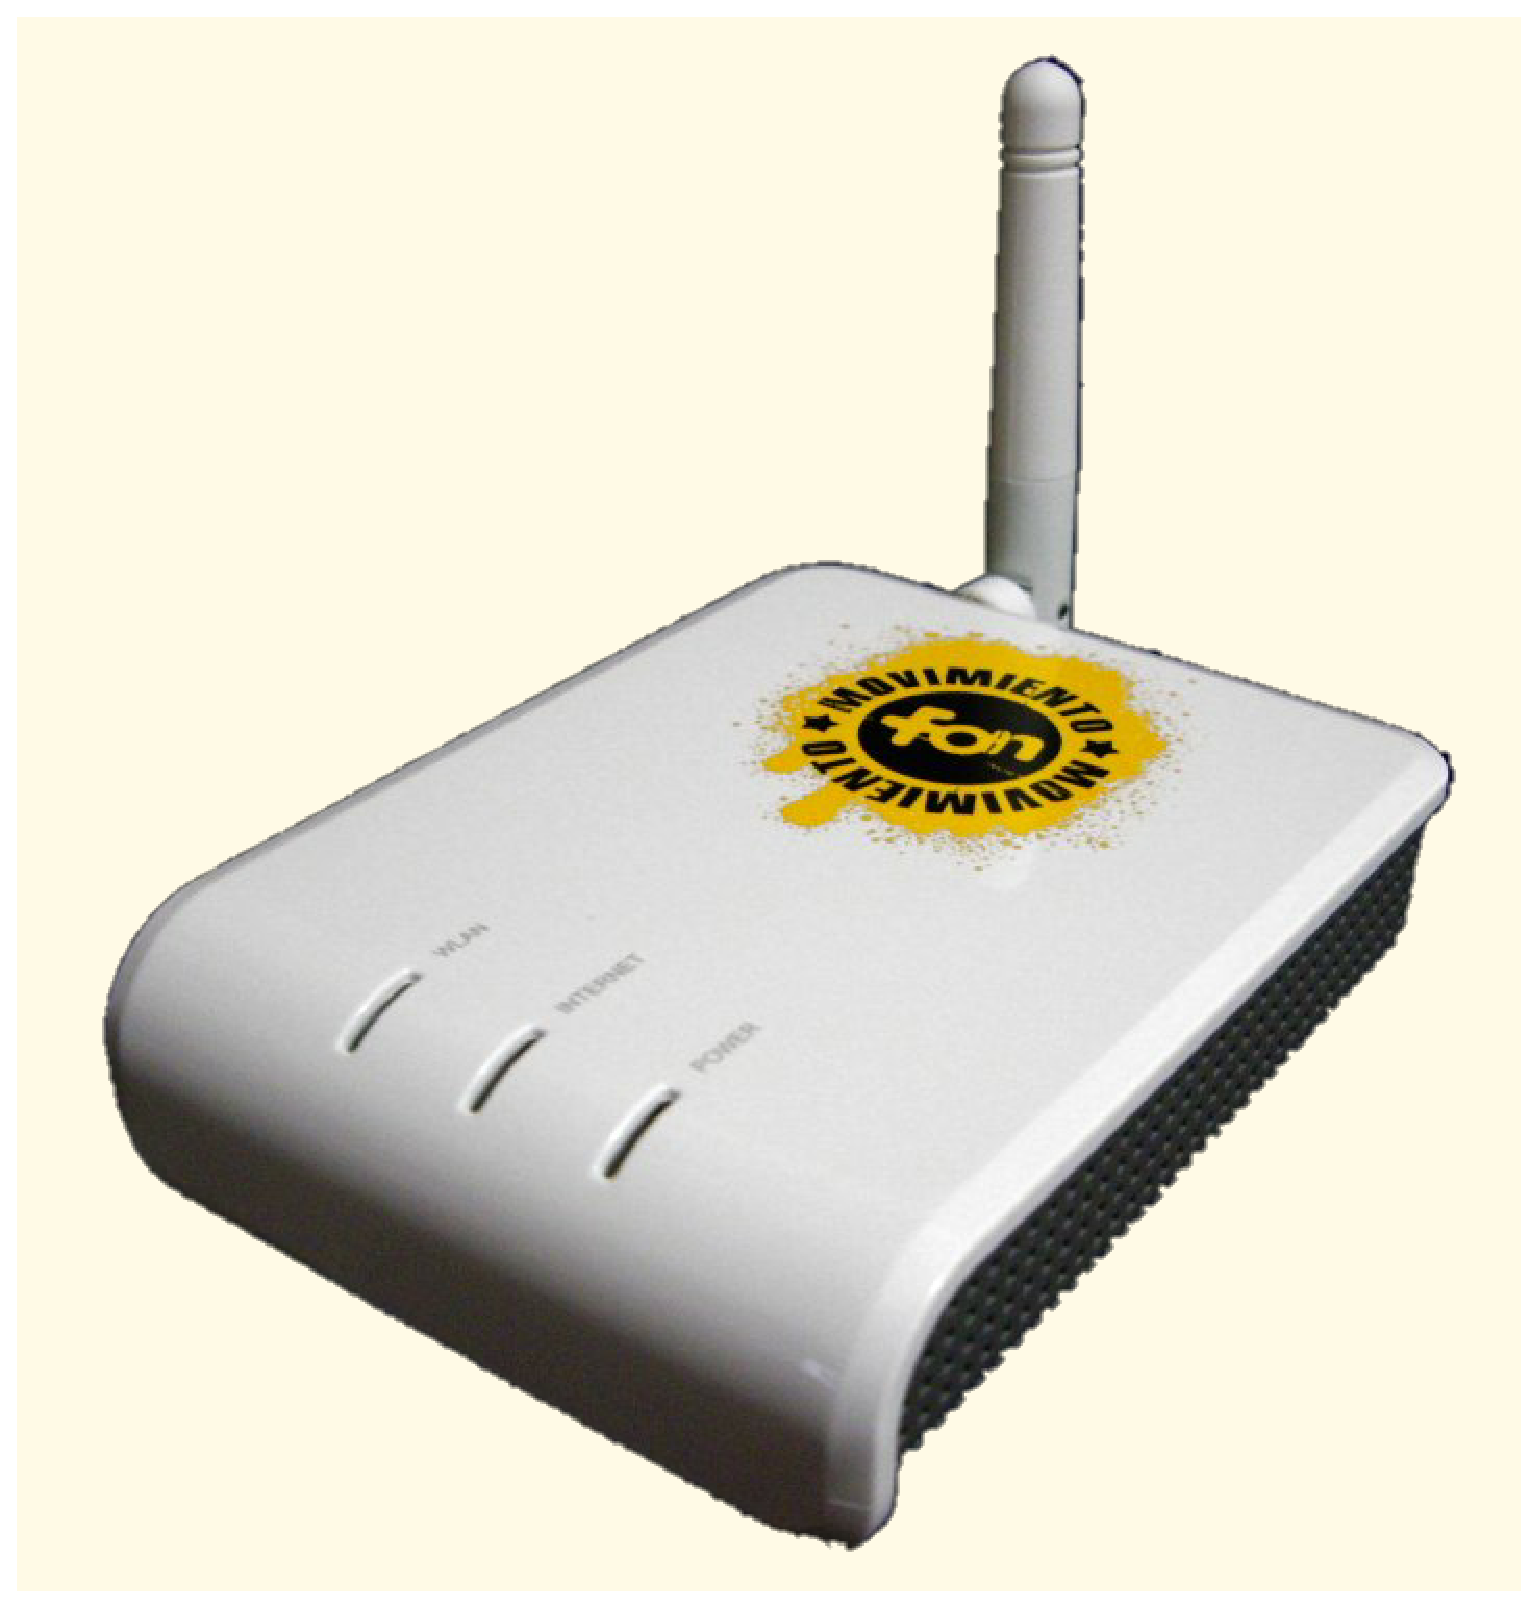
\includegraphics[keepaspectratio, width=0.2\textwidth]{images/lafonera-sourcewikipedia.eps}
  \\
  Figure 1. \textit{La Fonera's initial project router.}
\end{center}

\vspace{0.35cm}

A more recent project like Hotspot me!\cite{hotspotme}
and also very aligned with the technological demonstration
described in this document consist on using mobile
APIs to allow users to share WiFi hot-spot tethering
to users nearby in exchange for ETH supported by a
micro-payment channel contract.


\section{Technological background}\label{ch:bc}

\vspace{0.35cm}

Blockchain technologies support a ledger of records in
continuous growth called blocks.
They are linked and secured by
cryptography. Adopt the P2P protocol
(\textit{peer-to-peer}) in order to be distributed
with not a single point of failure.

\vspace{0.35cm}

The consensus mechanism ensures a common order
of unambiguous transactions and
blocks, and guarantees integrity and
blockchain consistency
through geographically distributed nodes.
By its design, the blockchain has characteristics
such as: decentralization, integrity and audibility.
The blockchain can serve as a new
type of software connector, which should be considered
as a possible decentralized alternative to storage
of existing centralized shared data.

\vspace{0.35cm}

In addition, depending on the different levels of
access permission, block chains can
split into two types:
1) public (such as Bitcoin and Ethereum); and
2) private (such as Hyperledger). Blockchain serves
as a platform for smart contracts
(hereinafter, \textit{smart contracts}).
For example, programmed in the Solidity language of
Ethereum that are able to be compiled into Ethereum
Virtual Machine bytecode and run over this EVM.
Blockchain is a technology concept
DLT distributed ledger
(\textit{distributed ledger technology}).
It can be integrated into multiple business areas.

\vspace{0.35cm}

Ethereum
blockchain is proposed as a first optimal candidate platform
to support this project PoC attending to
following reasons:

\begin{itemize}
\item Is the most used and mature
Turing-complete-programmable blockchain technology.
\item Supports high quality and audited
libraries in Solidity (most used smart contract language in Ethereum).
\item Developments on Ethereum can be deployed
over public (main or test-nets) or private/permissioned networks.
\item Unlike Bitcoin, Ethereum supports miner fees using gas
instead of directly ETH; this can mitigate the effects of
volatile crypto-currency price by adjusting gas price depending
on ETH value.
\end{itemize}

%% \textit{ETH-Paid hotspot provider} (E-Php).
%% \\
%% \\
%% \textit{Hotspot handler} (hh).
%% \\
%% \\
%% \textit{Upstream Internet Service Provider} (U-ISP).
%% \\

\section{Proof of Concept description}

\subsection{Architecture}
\label{ch:architecture}
\vspace{0.35cm}

In order to support the PoC a
Raspberry Pi 3 Model B (see figure 2) has been used
as a single board computer to host all the required software.
Tested operative system was OSMC\cite{osmc} (a Debian based
GNU-Linux flavor) mainly used as media-center.
A WiFi access point using
hostapd\cite{hostapd} daemon over Raspberry's WiFi chip-set.
Raspberry Pi was also connected using ethernet cable
to an optical fiber commercial router (\textit{see figure 2}).

\begin{center}
%\begin{figure}[h]
%  \centering
  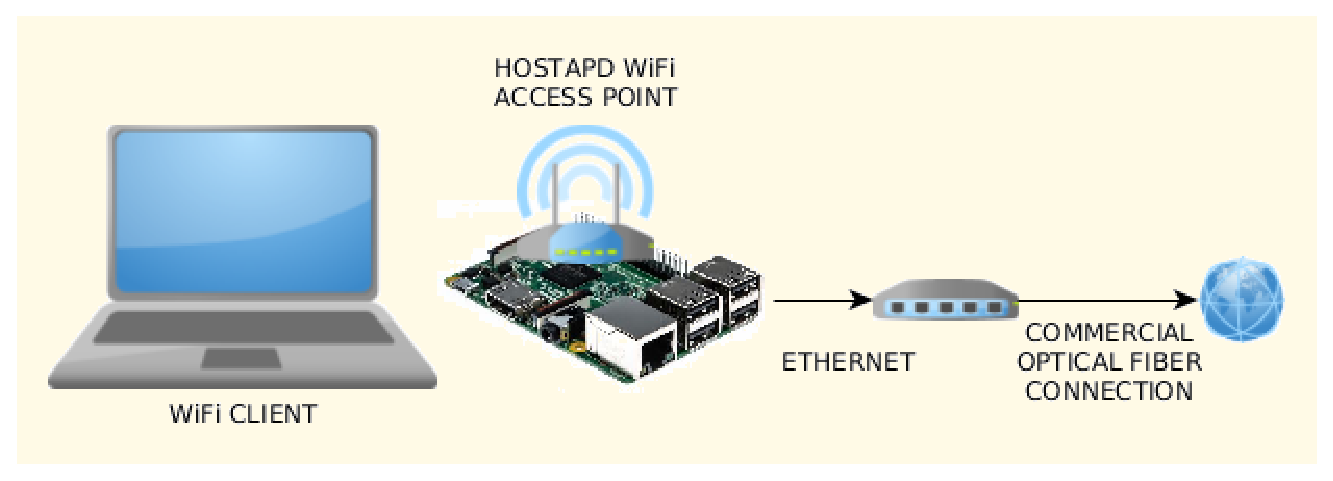
\includegraphics[keepaspectratio, width=0.5\textwidth]{images/physical-setup-y.eps}
%  \caption{Figura 2. Raspberry Pi 3 Modelo B. Fuente: [Raspberry 18]}
  %\end{figure}
\\
Figure 2. Physical Setup.
\\

\vspace{0.35cm}

% \begin{tabular} to 0.5\textwidth { | X[l] | X[r] | }
\begin{tabular}{ | m{0.125\textwidth} | m{0.3125\textwidth} | }
 \hline
 Specs & Raspberry Pi 3 Model B \\
 \hline
 CPU & Broadcom BCM2837, Cortex-A53 (ARMv8) 64-bit SoC @ 1,2 GHz \\
\hline
 RAM & 1 GB \\
\hline
 Connectivity & Wi-Fi 802.11 b/g/n (2,4 GHz) Bluetooth 4.1 Ethernet card up to 100 Mbps \\
\hline
 Ports & Full HDMI, 4 USB 2.0, MicroSD, CSI camera, DSI display \\
\hline
 Memory & MicroSD \\
\hline
\end{tabular}
\end{center}
\vspace{0.15cm}
Table 1. Raspberry Pi 3 Model B specs

\vspace{0.35cm}

Although it is not expressly indicated if it is free hardware
(\textit{open hardware}) or with trademark rights, on the
official website there's an explanation regarding
that Raspberry have distribution and sales contracts with
two companies and guarantee that anyone can become a re-seller or
re-distributor of Raspberry Pi cards\cite{RaspberryPi19}.

\vspace{0.35cm}

Dnsmasq\cite{dnsmasq} was used
as dynamic host configuration server for the wireless
network users and
iptables\cite{iptables} was used as a firewall running
both inside the Raspberry; by default, iptables
was configured to
drop all packet
forwarding traffic from users connected to the wireless
domain and at the same time to redirect all
traffic to Raspberry's HTTP port where a
captive portal was listening incoming connections.


\subsection{Main connection workflow}

\vspace{0.35cm}

Main idea is that the users can join freely
to the wireless hot-spot and access the web captive portal
(\textit{hosted on the same Raspberry}) application that
communicates with a back-end that controls iptables
rules and also an Infura light proxy able to relay RPC
calls arriving on 8545 port of the Raspberry.

\vspace{0.35cm}

To keep users' freedom to interrupt the service consumption
whenever they want and also avoid the overhead of transacting
many times with the smart contract; authors have implemented
what is known as a state channel in a smart contract; this
makes possible to keep control of the time fraction of the service
that's already consumed and at the same time cryptographically
guarantee that the smart contract is going to unlock the funds
when the provider desires to do so. State channels are a
standard pattern in most blockchain applications and in all cases
(\textit{independently of the complexity}) present three main
steps: opening, transaction and closing; project's particular implementation
described below:

\subsubsection{Channel opening}
The connection flow as shown in figure 3, can be summarized
as follows:

\begin{itemize}
\item[] 1) The user associates the laptop with the WiFi hot-spot.
\item[] 2) Once connected is redirected to the captive portal front-end.
\item[] 3) Front provisions MetaMask as Web3 provider.
\item[] 4) Front-end uses MetaMask to allow the user
  to send value to the contract
\item[] 5-6) Signed transaction is relayed through a light Infura proxy listening
  on port 8545.
\item[] 7) Once transaction is confirmed, the back-end iptables controller
  start forwarding user's traffic.
\end{itemize}


\subsubsection{Channel transactions}
Before sending the initial value transaction (\textit{proportional to
  the initially expected duration of the service})
user's front-end generates an ephemeral elliptic curve
secp256k1 keypair and sends the public key to the contract to open the state channel.
Corresponding ephemeral private key is the one that's going to be used
to periodically (each 10 s approximately)
produce increasing value signatures proportional to the
service consumption elapsed time. This signatures are being send to the
back-end instead of the blockchain; back-end verifies and validates the
signatures and stores the last one (\textit{the most valuable}).

\subsubsection{Channel closing}
At the end, when the connection time is exhausted or the back-end
stops receiving channel transactions for approximately 60 seconds,
the back-end sends the last seen transaction to the smart contract
using the method \texttt{closeChannel}; this method, when called
with a valid channel signature as parameter, unlocks user's original
funds and transfer the signed amount to the contract owner
(\textit{provider of the service}) and the corresponding return
to the user.

\begin{center}
%\begin{figure}[h]
%  \centering
  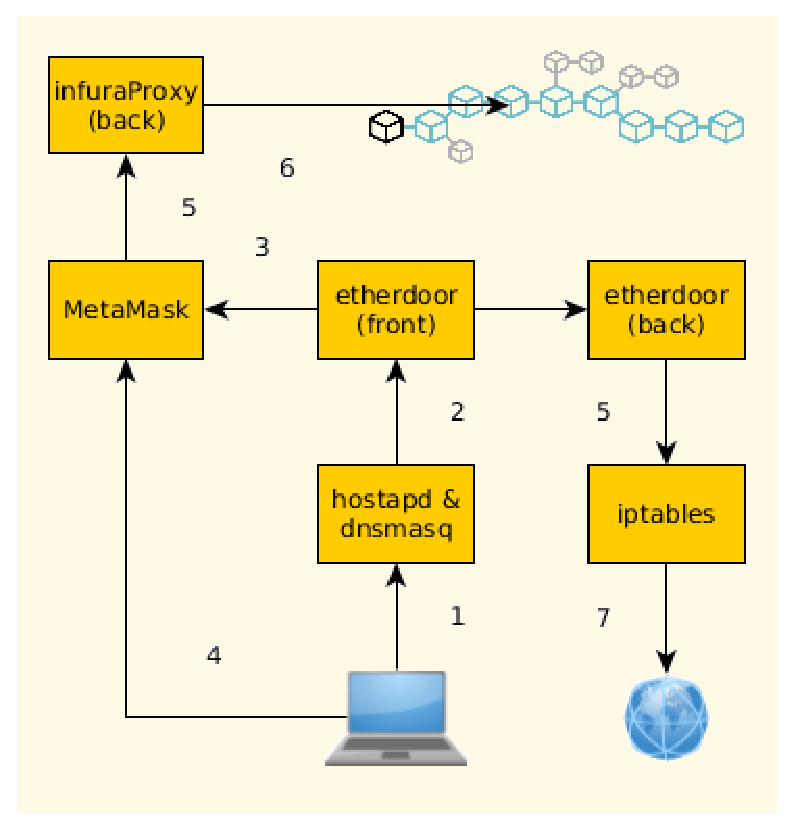
\includegraphics[keepaspectratio, width=0.5\textwidth]{images/con-flow-y.eps}
%  \caption{Figura 2. Raspberry Pi 3 Modelo B. Fuente: [Raspberry 18]}
%\end{figure}
\\
Figure 3. Connection work-flow.
\\
\end{center}

\begin{center}
%\begin{figure}[h]
%  \centering
  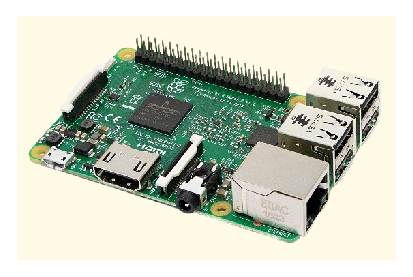
\includegraphics[keepaspectratio, width=0.2\textwidth]{images/rpi3modelb-sourceamazon.eps}
%  \caption{Figura 2. Raspberry Pi 3 Modelo B. Fuente: [Raspberry 18]}
%\end{figure}
\\
Figure 4. Raspberry Pi 3 Model B\cite{RaspberryPi19}.
\\
\end{center}

\subsection{Detailed software description}

\vspace{0.35cm}

This section includes a detailed rationale software description of all
the components and sub-components.

\subsubsection{Smart contract}

\vspace{0.35cm}

The smart contract\cite{state-channel-contract-a} used
to implement the proof of concept consists on a simple
uni-directional micro-payment channel that is Ownable
depending on OpenZeppelin contract; uses also OpenZeppelin's
SafeMath library in order to perform accounting operations
and finally uses also OpenZeppelin's ECDSA library to support
the signature validation on the closing channel operation.

\vspace{0.35cm}

Main data structure of the contract described below:

\vspace{0.35cm}

\paragraph{\texttt{ChannelData}} Includes payer Ethereum address,
its state channel ephemeral address, deposit amount, opening time
and a boolean representing the open/close status of the channel.

\vspace{0.35cm}

Contract's storage variables:

\vspace{0.35cm}

\paragraph{\texttt{channelCount}} uint256 variable that increments
in a unit every time a user opens a channel. This operation
does not rely on SafeMath since it's virtually impossible to
overflow an incremental
uint256 storage record according to transaction fees or block time delays.

\vspace{0.35cm}

\paragraph{\texttt{channelMapping}} Holding a key-value map between
channelCount values and channelData structures.

\vspace{0.35cm}

\paragraph{\texttt{pricePerSecond}} Constant keeping track of
service price per second.

\vspace{0.35cm}

The main methods of the smart contract:

\vspace{0.35cm}

\paragraph{\texttt{openChannel}} Receives as parameters, the ephemeral address
of the user and also the purchased service value.

\vspace{0.35cm}

\paragraph{\texttt{closeChannel}} Accepts the amount of ETH to
transfer to the contract owner, the channelId and the signature of the
payer; checks the signature, calculates the non used purchase value
and, after updating the state, transfers both the amount to the owner
of the contract, and the return to the channel opener

\vspace{0.35cm}


\paragraph{\texttt{claimTimeout}} Method that allows the payer to
close the channel in case contract owner does not close it after
some \texttt{expirationTime}.

\subsubsection{Etherwall}

\vspace{0.35cm}

Consists on a NodeJS back-end that fulfills three main system functions:

\begin{itemize}
\item Controls the state of the current connections.
\item iptables interfacing.
\item Micro-payment signature and amount validations.
\end{itemize}

On execution uses the module \texttt{lib/iptables.js}
to setup and initialize system's iptables redirecting
all 80 port traffic to Raspberry's
ip address; to do so, relies on the node module \texttt{child\_process}
to spawn system commands. Also redirects all traffic trying
to reach 8545 port to itself the same way in order to
redirect MetaMask's RCP calls to the lightweight infuraProxy\cite{infuraProxy}
developed also for this project and contained in etherwall's root directory.

\vspace{0.35cm}

After initializing, the back-end using the web framework\cite{express}
etherwall exposes the following endpoints:

\vspace{0.35cm}

\paragraph{\texttt{GET /generate\_204}} As a way to enable
captive portal detection to Android OS. HTTP Status 204
means the file exists but, is empty.
This lets Android know that the Internet is accessible.
If the request receives HTTP Status 302 (temporary redirect)
instead of HTTP 204, Android will follow the
redirection URL to display the Captive Portal to the user.

\vspace{0.35cm}

\paragraph{\texttt{POST /mac}} Endpoint to request a new
connection; mainly
accepts the time left to use the service as a parameter
and internally gets the MAC address of user's device
making an arp table query based on client's ip address.
After that invokes \texttt{lib/iptables.js} \texttt{grantAccess}
function in order to insert a rule to enable packet forwarding
for this particular MAC address on top of iptables.
Also uses module \texttt{lib/connections.js} to keep persistence
of the connection status. Once connected after posting
\texttt{timeLeft} to this endpoint, in module
\texttt{lib/connections.js} there's a \texttt{setInterval}
triggering getting connection status and time since last
micro-payment on a 5 seconds frequency. In case \texttt{timeSinceLastPayment}
exceeds 60 seconds or \texttt{timeLeft} goes negative,
disconnects the client deleting the forwarding rule from
iptables.

\vspace{0.35cm}

\paragraph{\texttt{GET /mac}} Retrieves the status of client's
connection from \texttt{lib/connections.js} module; this module
in addition, provides some serialized persistence using a JSON
file under the \texttt{data/} directory to keep state integrity
between server restarts.

\vspace{0.35cm}

\paragraph{\texttt{POST /payment}} Endpoint that allows the front-end
to send a payload containing a JSON body passing the corresponding
contract data:

\begin{itemize}
\item \texttt{channelId}
\item \texttt{amount} (to unlock)
\item \texttt{signature}
\end{itemize}

In order to verify the correctness of the payload, uses Web3
module to compute the \texttt{soliditySha3} and compares it
to the signature's \texttt{messageHash}; after that recovers
the public address from the signature and compares it to
the associated smart contract mapping structure based on its
\texttt{channelId}; if everything matches, it additionally checks
that the unlocked amount is approximately what it corresponds
taking into account connection elapsed time
(\textit{using a kind threshold of 60 seconds marginal cost});
in case everything is correct, stores the payment together
with a time-stamp as the last one corresponding
to the connection using again \texttt{lib/connections.js} module.
This is done to allow bootstrapped \texttt{setInterval}
on the previously described \texttt{POST mac/} to process
the timeout business logic.

\subsubsection{etherdoor} A very simple front-end based on React
using material styling; App's main \texttt{componentDidMount}
initializes the state including Web3 object and smart contract
wrapper, gets current connection status from back-end's
\texttt{GET mac} endpoint and creates the micro-payment
state channel ephemeral account; at the end triggers a
\texttt{setInterval} loop that when connection activates,
will be responsible of sending proper signed micro-payments.

\begin{center}
  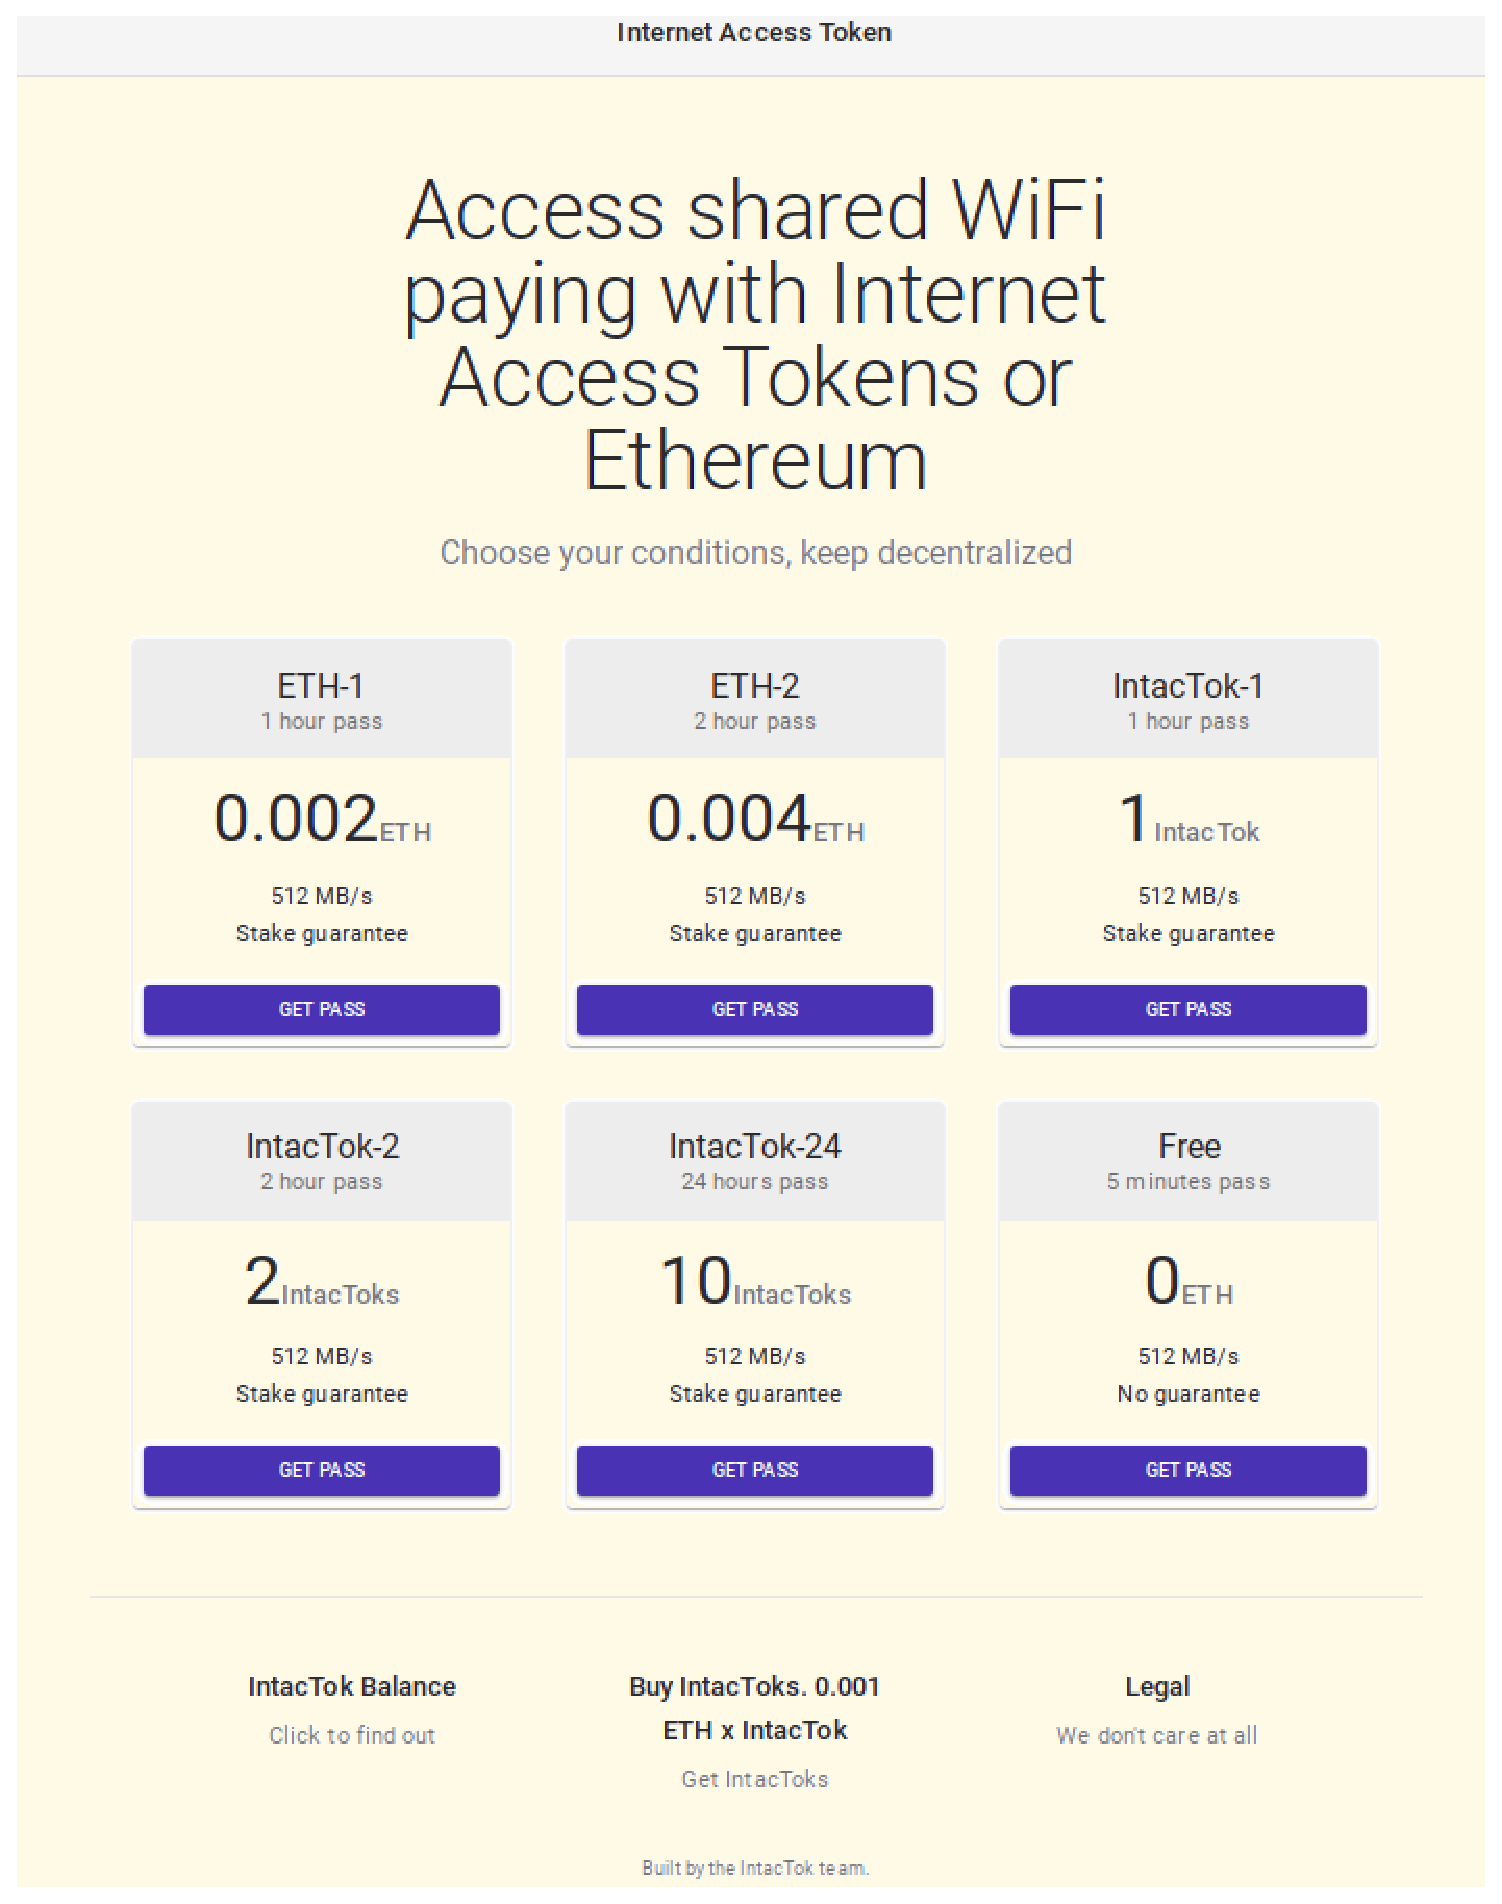
\includegraphics[keepaspectratio, width=0.4\textwidth]{images/portal-y.eps}
  \\
  Figure 5. \textit{Etherdoor front-end landing page}
\end{center}

Usage depends on some button clicking, triggering
\texttt{someMinutesPass} function invocation that launches MetaMask
as Web3 provider making possible to the user to open a channel
on the smart contract building a transaction and relaying it
through \texttt{infuraProxy}; it also invokes \texttt{startChannel}
that will update React's App state and will cause
\texttt{signMicroPayment} function to periodically on a 10 seconds
interval to sign and post to the back-end the increasing amount
micro-payments.

\section{Quality considerations}\label{sec:proofs}

\vspace{0.35cm}

To validate the PoC, a battery of tests has
been defined. For example, given
that smart contract normally handle money,
it is essential to ensure that
its number of failures and vulnerabilities is low\cite{Hegedus18}.

\subsection{State channel contract tests}

\vspace{0.35cm}

During development and in order to ease
the automatic deployment of the contract
over a Truffle's suite Ganache-CLI\cite{ganache}
instance there are two util scripts on the
repository\cite{state-channel-contract-a}
\texttt{utils/compile.js} and \texttt{utils/deploy.js}
that take care of merging all the Solidity source
code required and deploying it to the Ganache instance.

\vspace{0.35cm}

In repository\cite{state-channel-contract-a} module
\texttt{main.test.js} there are the following Mocha
framework\cite{mocha} based tests; tests use Chai assertion
library\cite{chai} using its \textit{should} mode whenever
possible but some of the assertions still have to be done
by \texttt{try-catch} pattern due to Chai not supporting
at the time of writing \texttt{BigInt} operation.

\vspace{0.35cm}

Non-trivial tests covering main work-flows include:
\begin{itemize}
\item Contract requires a minimum value amount to open a channel.
\item A user can open a channel sending value over a minimum amount providing
  in addition an Ethereum ephemeral public key
\item Prevention of channel closing operation using a different private key
  in signature.
\item Ability of the contract owner to close the channel using a properly
  generated user signature.
\item If channel is not closed by the owner, the user, cannot close it
  before a certain amount of time.
\item In case reaching expiration time without the owner properly closing the channel,
  the user can close the channel receiving initial payment amount.
\end{itemize}

\subsection{Front-end \& Back-end manual testing}

\vspace{0.35cm}

Both components were heavily manually tested, during development
in order to assure the correct work-flows were correctly supported.


\subsection{Static analysis}

\vspace{0.35cm}

To help developers and make technology more mature,
analysis tools\cite{ConsenSys19} were considered.

\vspace{0.35cm}

For this project, Mythril from ConsenSys was used. Mythril is a
security analysis tool for EVM (Ethereum Virtual Machine) byte-code.
It detects security vulnerabilities in smart contracts built for Ethereum.

\vspace{0.35cm}

Analysis was carried out over the Solidity-based smart contract called
StateChannel.sol.

\vspace{0.35cm}

The installation steps are as follows in:

\vspace{0.35cm}

https://github.com/ethereum-internet-access/mythril
Firstly, the local source code was analyzed:

\begin{verbatim}
$ cd contracts
$ myth analyze StateChannel.sol \
  > ./security-report
$ cat ./security-report
\end{verbatim}

\vspace{0.35cm}

Secondly, on-chain smart contract was analyzed.
Because the smart contract was deployed on Ropsten test-net,  executed:

\begin{verbatim}
$ myth analyze --rpc \
  infura-ropsten -a \
  contract_address \
  > ./security-report
$ cat ./security-report
\end{verbatim}


\subsubsection{Analysis tools outcome}

\paragraph{Dependence on predictable environment variable}

Both Mythrill and Manticore have reported a low severity warning located on function
\textit{claimTimeOut}, due to the use of the special variable \textit{block.timestamp}, -refered
to as \textit{now}.

Mythril states:

\textit{A control flow decision is made based
on a predictable variable. The block.timestamp environment variable is used in to determine
a control flow decision. Note that the values of variables like coinbase, gaslimit,
block number and timestamp are predictable and can be manipulated by a malicious miner.
Also keep in mind that attackers know hashes of earlier blocks. Don't use any of those
environment variables for random number generation or to make critical control flow decisions.}

\vspace{0.35cm}

This warning is considered assumable due to this two facts: 1) the tiny incentive for the
malicious miner, who merely could steal the few \textit{weis} value of a channel in favour
of the \textit{user}, and 2) the uncertainty of reaching the goal of claiming the refund
before the contract owner closes it.

\vspace{0.35cm}

\paragraph{Multiple Calls in a Single Transaction}

Mythrill also reports this low severity warning located on function \textit{closeChannel}:

\textit{Multiple calls are executed in the same
transaction. This call is executed after a previous call in the same transaction.
Try to isolate each call, transfer or send into its own transaction.}

\vspace{0.35cm}

A workaround in order to avoid this issue couldn't be found, due to the fact that both
transfers must be done and for the low amount of value
allowed in implied transactions authors preferred
the push over pull pattern to avoid on-chain transaction overhead.
In the \textit{Writing a Simple Payment Channel} example available in
\href{https://solidity.readthedocs.io/en/latest/solidity-by-example.html#micropayment-channel}{Micropayment Channel},
a \textit{selfdestruct} is proposed. But in this project, a single smart contract is expected
to support several channels, rather than deploying a fresh contract in every connection.
Furthermore, both calls to \textit{transfer} happen after any changes to state variables,
so the contract is not vulnerable to a reentrancy exploit.

\paragraph{Beyond the scope of a PoC}

Some improvements should be considered prior to taking the \textit{StateChannel.sol}
implementation beyond the scope of this PoC:
\begin{itemize}
\item a setter function for \textit{pricePerSecond} should be in place. However, for the sake of
fairness, nobody should be allowed to update the price after the channel is opened. So therefore,
a new atribute storing the current channel price should be added to the \textit{ChannelData} struct.
\item minimal price allowed in channel openning should be a variable, rather than a hardcoded value.
\item only accepting ETH is a hard constrain that probably will frustrate any chance of a massive
adoption of this offering: ERC20 tokens should be considered.
\end{itemize}

\section{Deployment}\label{sec:deploy}

\vspace{0.35cm}

Docker is a tool that allows you to deploy applications
inside of software containers. This can be useful for our
Raspberry Pi because it allows users to run applications with
very little overhead, as long as the application
is packaged inside of a Docker image.

\vspace{0.35cm}

To do so, simply install Docker and run the container over Raspbian/ARM.
It would deploy project's software. The script to execute is as follows:

\begin{verbatim}
$ sudo apt-get update
$ sudo apt-get upgrade
$ sudo apt-get install curl
$ curl -sSL \
  https://get.docker.com | sh
$ sudo apt-get install git
$ git clone \
  https://github.com/ \
  ethereum-internet-access/docker.git
$ cd docker
$ sh ./install-project\
  -inside-docker-container.sh
\end{verbatim}

\section{Security considerations}

\subsection{Network security}

\vspace{0.35cm}

Network security of the PoC depicted in this work
has some issues having to do with the ability of
an attacker to associate to owner's network without
any authentication nor authorization protocol; taking
this into account, special care has to be taken to
properly secure any attack surface:

\begin{itemize}
\item Add firewall rules to prevent IP traffic between
  different end users.
\item Obviously safe the connectivity to the Raspberry
  using a wire connection and filtering any traffic on 22 (ssh)
  port coming from the wireless interface.
\item For this PoC, the captive portal IP address was used; because of that,
  TLS was not supported; accordingly the user had no guarantee of
  authenticity of the WiFi service provider.
\end{itemize}

\subsection{Cryptographic security}

\vspace{0.35cm}

All smart contract-blockchain transactions are being processed
using Infura as an Ethereum proxy; main potential
security issue regarding
private key management arises when considering the ephemeral
private keypair generation on the front-end. Since this key
is not managed by MetaMask is not isolated from browser's
JavaScript engine being vulnerable to plain HTTP malicious
attacks by third parties and cross-site scripting issues.

\subsection{Security summary}

\vspace{0.35cm}

Apart from issues considered previously, general considerations
regarding safety of the system should take into account
the amount of value implied in the transactions;
being these micro-payments and not big amounts of value nor
big investments either, system can be considered relatively
safe in proportion to the assets (\textit{small Ethereum amounts})
transacted.

\section{Regulation status}
\vspace{0.35cm}

Any organization that has customers on the premises,
from coffee shops to libraries, might want to offer free (or even
paid-for) Wi-Fi as an attraction. Collecting and storing personal
information brings responsibilities under European Union’s General
Data Protection Directive (GDPR). The GDPR\cite{gdpr16}, which took
effect on 25 May 2018, applies to any organization that handles EU
residents’ personal data. From 25 May on, however, organizations
failing to comply with the regulation face fines of up to 4 \% of
their global turnover. There are Certified EU General Data Protection
Regulation Foundation (GDPR) Training Courses.

\vspace{0.35cm}

Another look at the major obligations imposed by this
regulation can be considered\cite{tata17}:


\vspace{0.35cm}
1. ART 5/1B and 1C - DATA MINIMIZATION:
Prohibited is the collection of more data than that required for the
adequate purposes for which it is being processed. For instance, if
you offer restaurant guests free WiFi access it is not necessary to
ask for their address data in this connection. However, if you are
interested in finding out where your guests are from - which can be a
completely legitimate interest for a restaurant owner to have - you
are indeed entitled to pose the question, but your guests must divulge
the information consciously and voluntarily and perhaps you should
only ask them for their postcode.

\vspace{0.35cm}
2. ART 5/1E - STORAGE LIMITATION:
Data may not be stored for longer than is necessary for the purposes
for which the data is being processed or than is necessary to meet
legal requirements.

\vspace{0.35cm}
3. ART 5/1A - LAWFUL, FAIR AND TRANSPARENT DATA
PROCESSING: Data subjects have a right to know what their data is
being used for and must be able to rely on the fact that it will not
be used for other purposes. This is why coupling of information is
prohibited. Collected data may only be used for the agreed purpose –
for example, to allow restaurant guests to use the in-house
WiFi. Hence, the coupling of the provision of WiFi access to a
compulsory subscription to a newsletter is no longer permitted. You
are naturally permitted to invite your guests to subscribe – but you
will need to do so separately and in an obvious manner.

\vspace{0.35cm}
4. ART 5/2
and 30 - ACCOUNTABILITY AND RECORDS: The GDPR requires that everyone
dealing with personal data must maintain records of the processing of
this data and be able to demonstrate that the corresponding processing
activities conform to legal requirements. Hence, they must document in
a data processing register which categories of data are collected from
which categories of person and how the data is processed. Are you
processing the data in-house or is the task outsourced to a service
provider? Is data transferred to a country outside of the EU? If so,
does the destination country provide a level of data protection
equivalent to that in the EU? This is perhaps the most problematic
aspect because even if you outsource processing or use a Cloud service
provider you are still held responsible for ensuring legal compliance
with regard to what happens to any data obtained from subjects.

\vspace{0.35cm}
5. ART 5/1F and 28 - INTEGRITY AND CONFIDENTIALITY: You must ensure
appropriate security of data and also ensure that it cannot be
tampered with. But how do you do that? What if hackers launch a
malicious attack? Don’t worry; even government websites are not immune
to this sort of thing and it would be hardly fair if the GDPR were to
impose more stringent requirements on you. However, you are required
to put appropriate technical or organizational measures in place that
provide adequate protection of your customers’ data. The GDPR does not
spell out in so many words what these required ‘measures’
are. However, you can be certain that you will be at least be expected
to have a valid SSL certificate for your data-collecting website and
to conclude instruction and confidentiality agreements with your
personnel who come into contact with the corresponding data.

\vspace{0.35cm}
6. ART
12, 13 and 15 - INFORMATION AND RIGHT OF ACCESS: You are obligated to
provide information at any time to data subjects whose data you
process. This information and your data privacy policy must be written
in clearly comprehensible language and include a contact option for
data subjects.


\vspace{0.35cm}

In addition, the Proposal for a new ePrivacy
Regulation was tabled in January 2017, when GDPR was not yet
applicable and the European Electronic Communications Code\cite{eecc18}
was still being negotiated. Now, GDPR has been implemented,
changing many of the approaches and behaviors that the ePrivacy
Regulation aims to tackle. Additionally, the new EECC already ensures
an extended definition of what an e-communications service is, thereby
achieving one of the purported goals of the ePrivacy Regulation, which
is to broaden the scope of application of confidentiality obligations
to a larger number of Internet-based players.


\vspace{0.35cm} Because of these issues, good advice for anyone
planning to set up a hot-spot would be to collect as little personal
data from users as possible, and to think of any additional collection
as a potential liability.

\section{Further steps}

\subsection{5G Technologies and scarcity model}
\vspace{0.35cm}

In the recent years blockchain technologies
and in particular smart contracts have made possible
an innovative way to rule business and
processes between organizations.

\vspace{0.35cm}

One of the main application of smart contracts
consist on modeling a scarce resource representing
it using fungible (or not) tokens; in addition
to this, smart contracts can be programmed
to suit any possible business intelligence
according to rules well known and accepted
in advance by the parties transacting.

\vspace{0.35cm}

In the case of 5G technologies for practical reasons
and the high density of antennas required,
different operators shall be able
to dynamically share the same resources (i.e. neutral host
infrastructure)\cite{neutral}. At the same time
in order to manage
service operation efficiently through its whole
life-cycle there's the need to automate as much as
possible all the work-flows; this requirements
perfectly fit smart contract capabilities
to model and operate over a defined set of rules
supporting payments, escrows, rewards or penalties
depending on different conditions.

\end{multicols}
\begin{center}
%\begin{figure}[h]
  %  \centering
  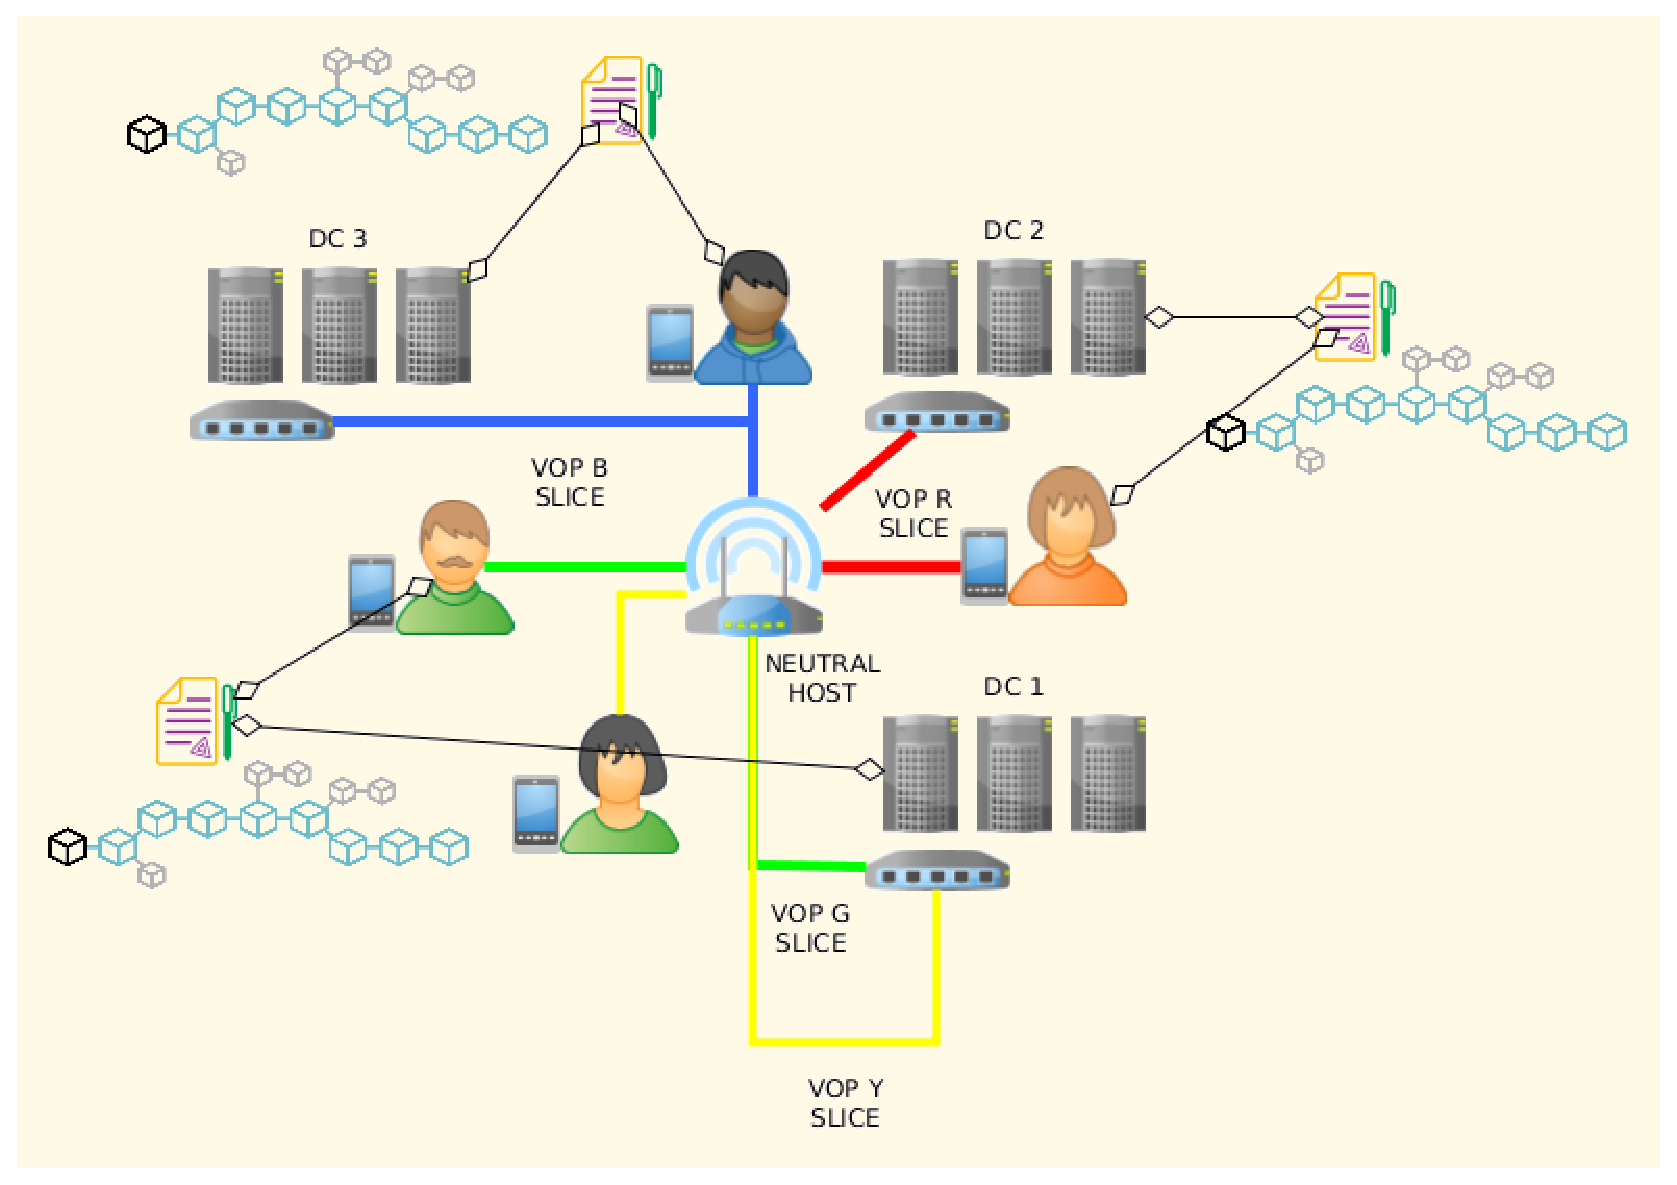
\includegraphics[keepaspectratio, width=0.8\textwidth]{images/bc5g/slices-y.eps}
%  \caption{Figura 2. Raspberry Pi 3 Modelo B. Fuente: [Raspberry 18]}
%\end{figure}
\\
Figure 6. Slicing model.
\\
\end{center}
\begin{multicols}{2}

As an example, in figure 6 it is depicted how three virtual operators over
different infrastructures shared or not in a slice-model of a neutral host
infrastructure provide their service;
a slice can be described as a dynamic multi-tenant virtualization
of some physical resources like access points,
physical switches, routers and data-centers including mobile edge computing
appliances; this is the case of currently ongoing projects like
5GCity\cite{5gcity} where a distributed cloud
and radio platform for municipalities and infrastructure owners acting
as 5G neutral hosts is being developed and tested. Platforms
targeting 5G business models such as 5GCity can benefit from adding
this smart contract business logic in order to bill end-users and automate
all the accounting layer.

\vspace{0.35cm}

Main motivation to include a smart contract approach to the 5G
business model has direct correlation with securing and
automating all economical transactions according some pre-established
set of rules. In addition, automating as much as possible the
accounting and KyC layer relying on blockchain accounting smart
contract and identity systems (using blockchain as a Public Key
Infrastructure) can impact on a huge reduction of the overhead costs
of operators and neutral host providers lowering entrance barriers and
reducing market's friction.  This way, all the actors implied can
reduce bureaucracy costs and focus on their main activities providing
innovative good quality services to their customers and at the same
time keep a high standard regarding transparency and flexibility.

\subsection{Know your customer issue}

\vspace{0.35cm}

Although this is a promising approach; there's an issue with it regarding
regulation, in particular in the European Union, there's the requirement
that a telecommunication service provider must know their customers; this
is required for example to allow court requirements of users identity
in case there's some investigation of illegal activities. As a single payment
system, state channel smart contracts are pseudo-anonymous hence do not
support the \textit{Know Your Customer - KyC} required by regulation.

\vspace{0.35cm}

To take into account the problem illustrated in previous paragraph
a model of self-sovereign identity\cite{allen} can be taken as a basis
and in particular the one recently announced by the authorities
of Catalonia's government\cite{identicat} that will provide credentials
to citizens using DLT technologies as a Public Key Infrastructure; this
model could allow in some near future to give the citizen the option
of registering identity in such a way that her/his credentials can be linked
to some certified database that could be queried only by a judge
requirement and guarantee the users identities are recognized
%% and at the
%% same time hidden from service providers, discharging them from
%% any GDPR responsibilities apart from the intrinsic service provision
%% metadata.

\end{multicols}

\begin{center}
%\begin{figure}[h]
  %  \centering
  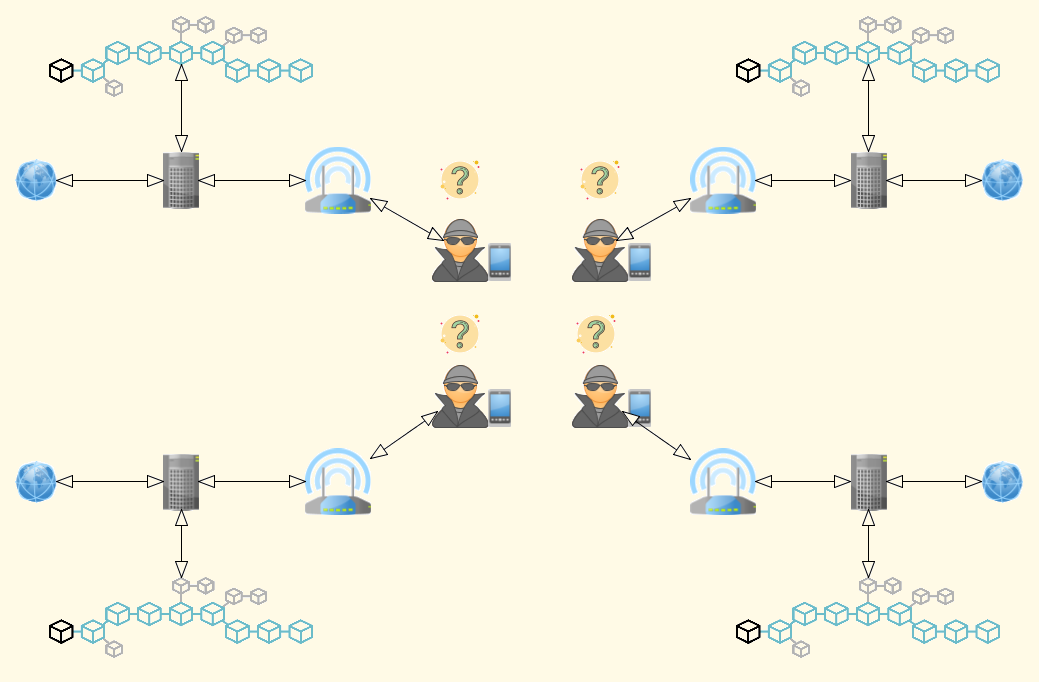
\includegraphics[keepaspectratio, width=0.8\textwidth]{images/bc5g/bc5g-y.eps}
  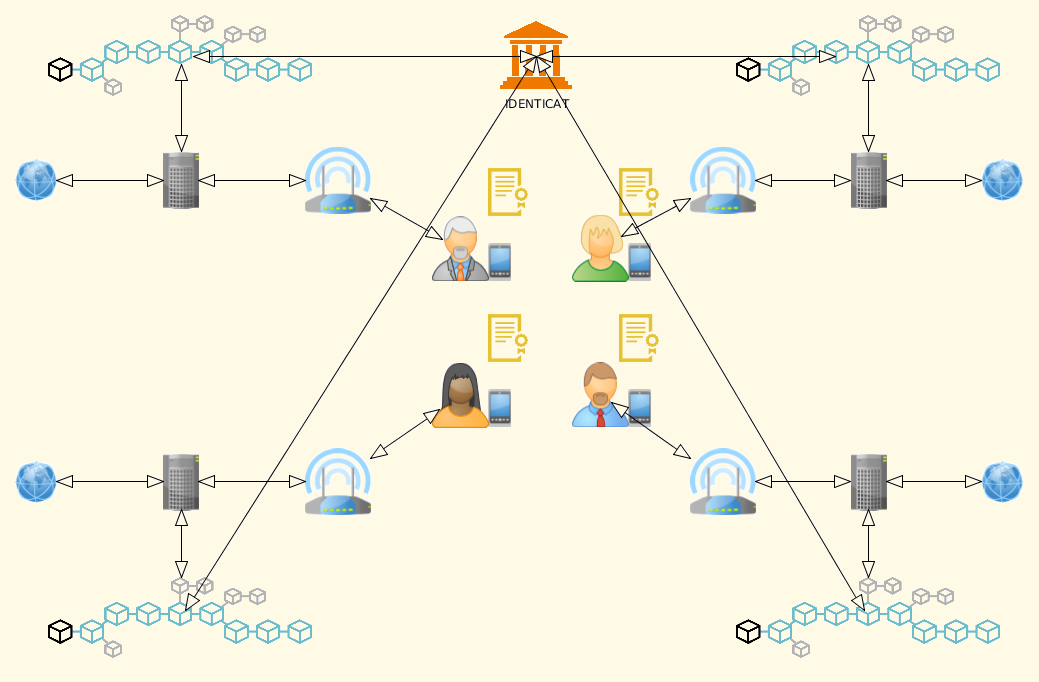
\includegraphics[keepaspectratio, width=0.8\textwidth]{images/bc5g/bc5g2-y.eps}
%  \caption{Figura 2. Raspberry Pi 3 Modelo B. Fuente: [Raspberry 18]}
%\end{figure}
\\
Figure 7. Upper figure shows a scenario where different users connect
to antennas controlled by a state channel smart contract like the one
described in this thesis; users remain pseudo-anonymous and hence, the
schema is not regulation compliant regarding the KyC that a
telecommunications
operator should guarantee in case of legal issues. On the other hand,
relying on a self-sovereign decentralized identity, bottom figure shows
up how the citizens can authenticate themselves to the system with the
guarantee there's a public administration validating their identities.
\\
\end{center}

\begin{multicols}{2}
by a public administration; this way, the service provider (\textit{in
  our case a telecommunications operator}) does not need to know
anything about a customer apart from a public key and a valid
credential signed by some recognized administration. This schema could be a real game
changer regarding operators market competition since they get rid-off
from several and costly processes that do not add any value to the service
they provide:

\begin{itemize}
\item Fully automated accounting and billing layer.
\item Regulation compliance without KyC on-boarding process.
\item GDPR compliance by default. Operator does not need to know
  user's name, bank account, etc.
\end{itemize}

\subsection{Instant portability}

\vspace{0.35cm}

This approach to the way customers interact with telecommunication
operators relying on a publicly recognized self-sovereign identity
can support a new way of handling portability granting full customer
empowerment when they want to switch from one operator to another;
in figure 5, is represented a process where a user opens a channel
in operator's A smart-contract; after that begins transacting with
this first operator paying as he/she consumes the access service
sending micro-payments to the operator.

\vspace{0.35cm}

After that, user decides to switch to a second operator, opening a channel
over operator B's contract; since operator A stops receiving the signed
micro-payments, opts for closing the channel back-drawing the earnings in operator's
account and return unexpended value to the user. Such kind of process can be accomplished
in a matter of seconds for a few cents fee literally obliterating any
operator lock-in mechanism thus supporting a really zero friction service market.

\end{multicols}


\begin{center}
%\begin{figure}[h]
  %  \centering
  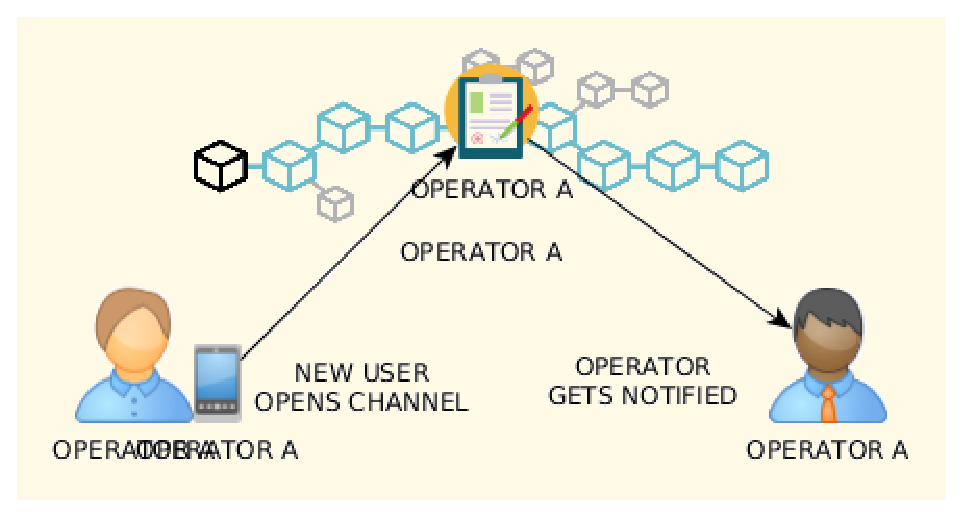
\includegraphics[keepaspectratio, width=0.6\textwidth]{images/bc5g/sc1-y.eps}
  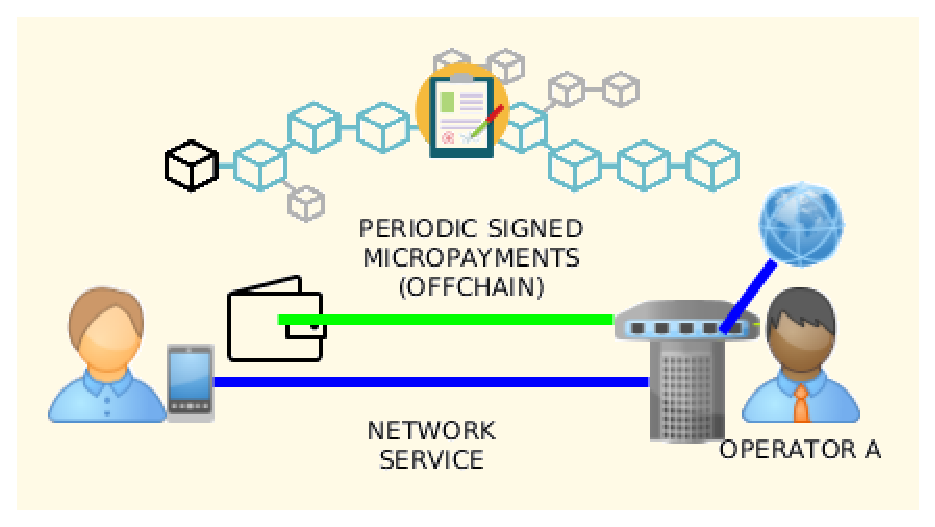
\includegraphics[keepaspectratio, width=0.6\textwidth]{images/bc5g/sc2-y.eps}
  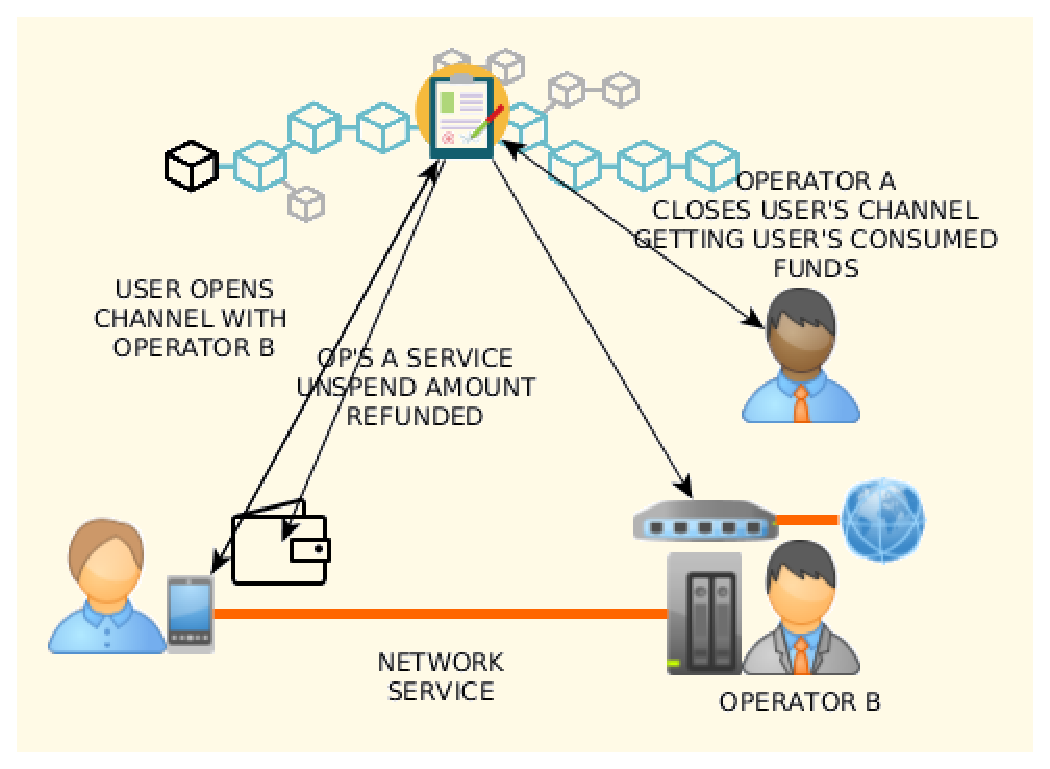
\includegraphics[keepaspectratio, width=0.6\textwidth]{images/bc5g/sc3-y.eps}
%  \caption{Figura 2. Raspberry Pi 3 Modelo B. Fuente: [Raspberry 18]}
%\end{figure}
\\
Figure 8. State channels support instant portability
between different operators with minimal fee.
\\
\end{center}
\begin{multicols}{2}

  \subsection{Towards telco market full tokenization}

  \vspace{0.35cm}

  This model can be extended without limits towards a full wireless
  telecommunication market tokenization; as depicted in figure 7,
  from the spectrum auctioning, including infrastructure providers
  virtualizing their appliances for virtual operators, end to users
  service provision and accounting relying on a self-sovereign
  identity system.


\end{multicols}
\begin{center}
%\begin{figure}[h]
  %  \centering
  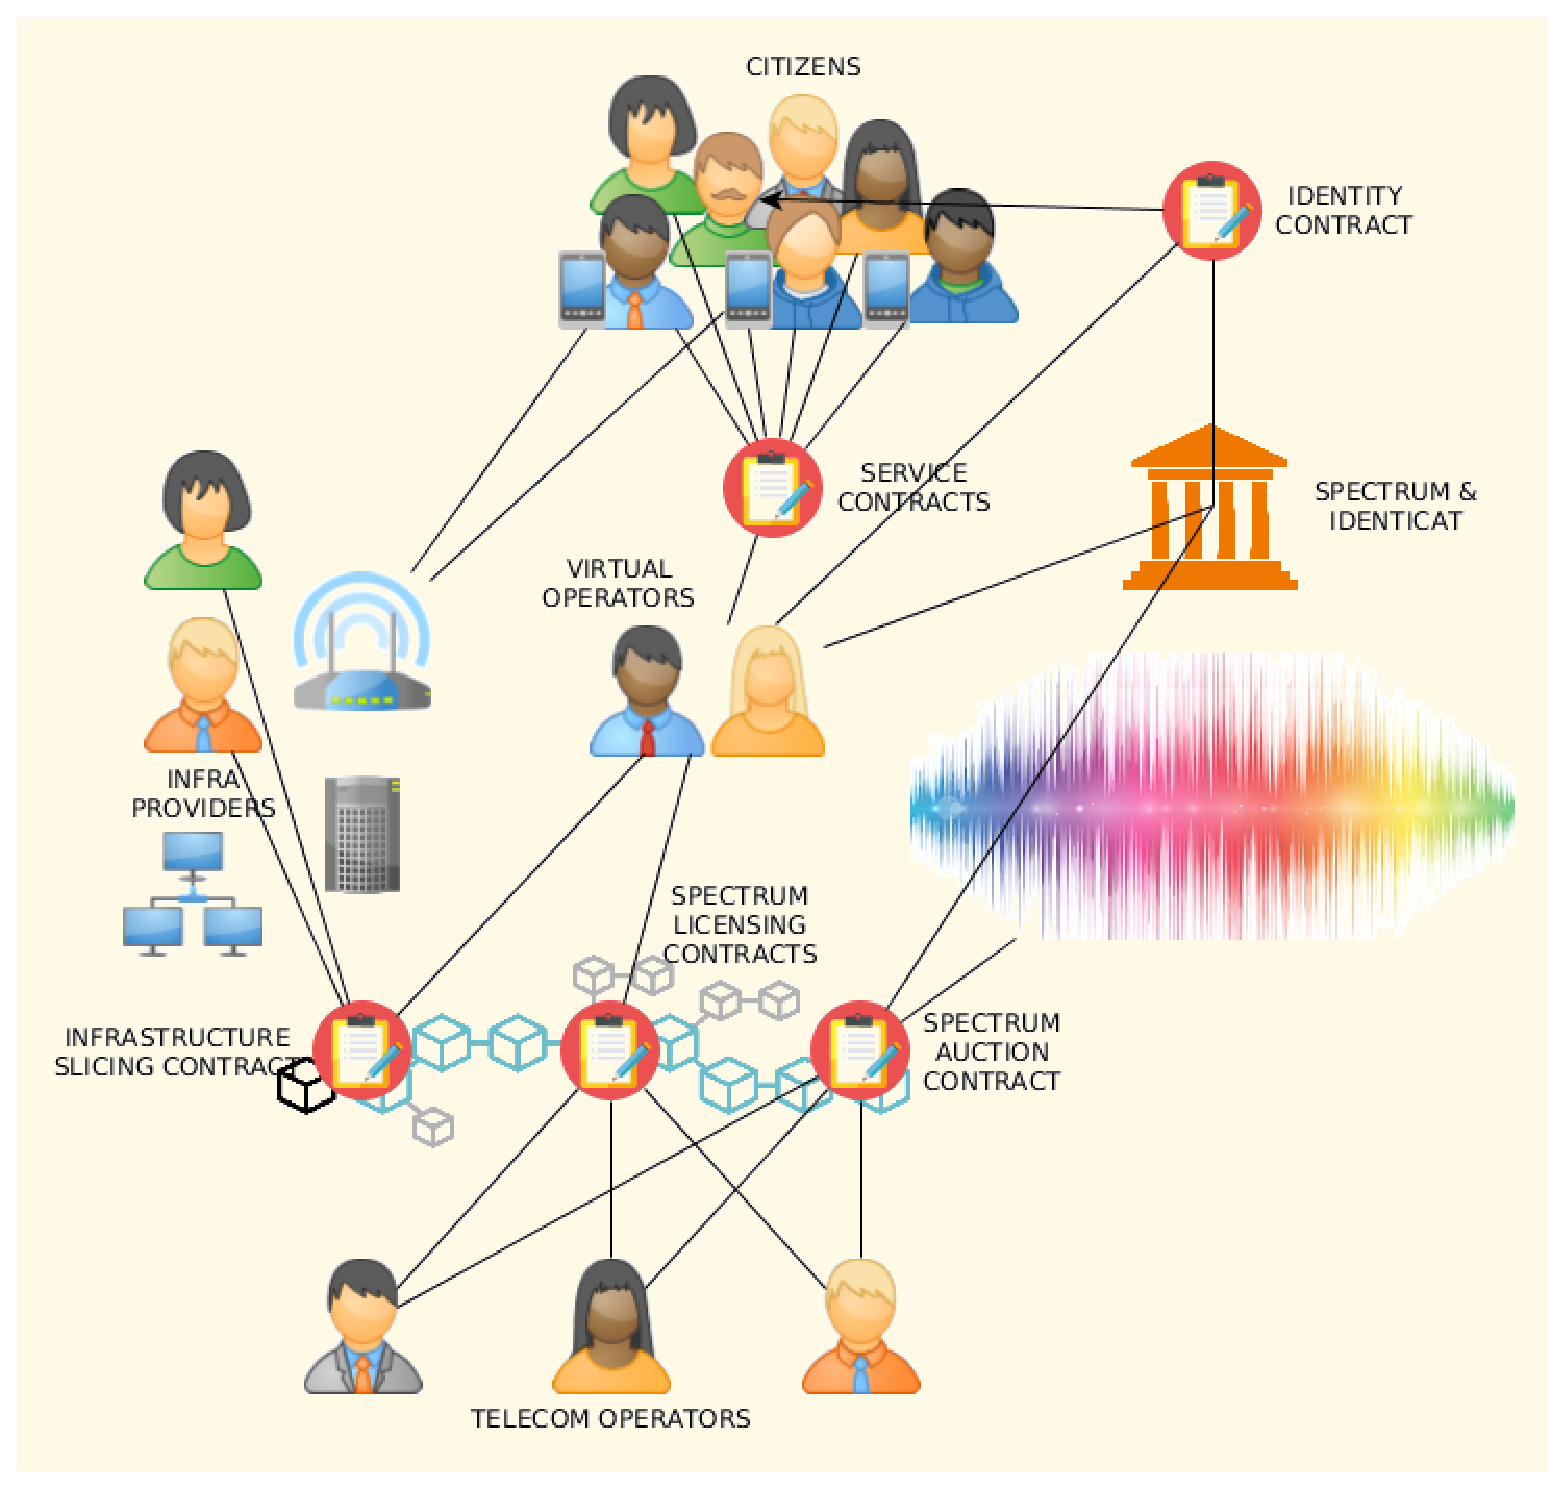
\includegraphics[keepaspectratio, width=0.8\textwidth]{images/bc5g/beyond-y.eps}
%  \caption{Figura 2. Raspberry Pi 3 Modelo B. Fuente: [Raspberry 18]}
%\end{figure}
\\
Figure 9. Full tokenization of wireless services from
the spectrum licensing to the citizen.
\\
\end{center}
\begin{multicols}{2}


\subsection{Risk analysis and mitigation strategies}

\subsubsection{Smart contract vulnerabilities}

Due to blockchain immutability, smart contracts cannot be updated once
deployed to the network; hence it's of critical importance to audit
before launching them to support economical transactions. Apart from
a detailed independent external and public audit,
there are several recognized good practices to avoid
vulnerabilities:

\begin{itemize}
\item Contract migration: as an emergency strategy to move assets from
one contract to another one, correcting the vulnerability.
\item Proxy contract pattern; a catalog contract pattern could support eventual
re-directions to different contract versions that can be upgraded
according to some defined governance (multisig between parties implied).
\item Check-effects-interaction pattern: Avoid returning execution flow
with pending state updates hence this can be an open door
to re-entrancy attacks.
\item Pull-over-push: perform accounting on-chain asset transfers and require
user intervention to withdraw tokens from the system.
\item Automated exhaustive testing with full code coverage.
\end{itemize}


\subsubsection{Regulation issues}

Blockchains, specially public ones are subject of several controversy
regarding regulation compliance; regulations like GDPR for data protection
and privacy and eIDAS regarding digital signature present some friction
at some aspects of blockchain based solutions; also, there's the
smart contract figure regarding how can it be legally binding
in order to ensure solutions built
for the project are 100\% European regulation compliant;
it's recommended to study implications
until having a clear guarantee that all features supported are legally
feasible on a final chosen deployment environment.

\subsubsection{Market collusion}

The potential transparency that a blockchain system makes possible can
lead to some risks having to do with market collusion and
the cooperation between different firms.
This cooperation may lead to a restrain of market competition,
in any of its forms, which translates into higher
profits for the firms in detriment of other parties benefits.
A cartel is an example of firms belonging to
the same industry structure which collude to some degree in
setting prices and/or output levels. According to that,
there's the need to analyze this potential risks ensuring
the design of reward/penalty schemes applying game theory and
mechanism design to
guarantee a fair competition market as outcome.


%% \section{Viabilidad de negocio}\label{sec:business}
%% (Por completar)
%% Comento el tema viabilidad de negocio porque ya está discutida
%% en Further steps

%% \subsection{Regulation considerations} \label{ch:regulation}

%% \vspace{0.35cm}

%% TODO; talk about GDPR, telco KyC, european market regulation, etc.

\section{Conclusions}\label{sec:conclusions}

\vspace{0.35cm}

World today is interconnected and wireless
internet access has a fundamental role. In this project
a Proof of Concept has been build. This PoC based in
commodity free hardware asset (Raspberry Pi) can serve
as an example of end-user wireless provision pay-as-you-go
using a state channel Solidity smart contract; KyC issues
and identity consideration have been discussed also leading
to the conclusion that complementing this approach with
what a self-sovereign identity can provide there's no need
to a telecommunication operator to perform a KyC process
in order to provision a service to a client.

\vspace{0.35cm}

On the other hand, one of the major problems with this approach has to do
with ETH-fiat exchange volatility
(\textit{see figure 7}), anyway, including
a feature to regulate minute price in the state channel
contract and taking into account gas prices can adjust
in order to properly
represent computation, bandwidth and storage costs this
problem can be completely avoided.

\section{Repository}\label{sec:repository}

\vspace{0.35cm}

Recommendations for further study as well as all of the source code generated in the project are also provided.
\newline\newline
Source code published in GitHub (public software repository) under MIT license:
\newline\newline
\href{https://github.com/ethereum-internet-access}{https://github.com/ethereum-internet-access}
\newline\newline
A demo video subtitled is available at the following address on YouTube:
\newline\newline
\href{https://www.youtube.com/watch?v=C9pVMn-pu_8&hd=1}{YouTube video demo}


\begin{center}
%\begin{figure}[h]
%  \centering
  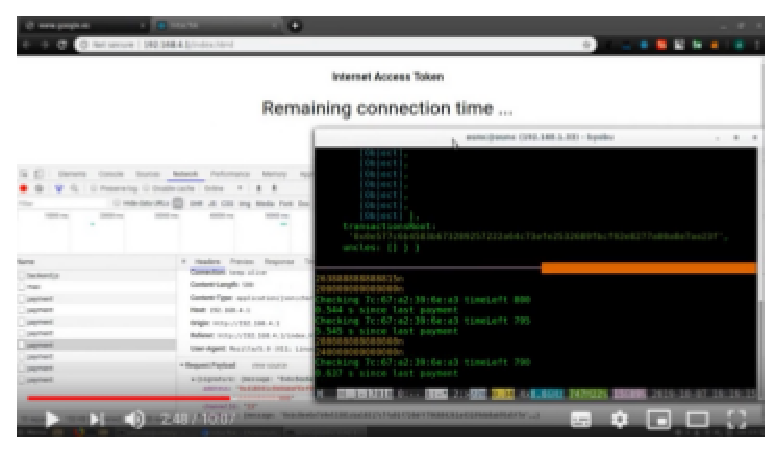
\includegraphics[keepaspectratio, width=0.5\textwidth]{images/maxresdefault.eps}
%  \caption{Figura 2. Raspberry Pi 3 Modelo B. Fuente: [Raspberry 18]}
%\end{figure}
\\
Figure 10. A demo video screenshot.
\\
\end{center}
\vspace{0.15cm}
Finally, the following addresses on Etherscan show the Ethereum transactions done:
\newline\newline

\begin{itemize}

\item \href{https://ropsten.etherscan.io/address/0x41b301c0b0abbfeef99803c23a281712e29b6ef1}{The contract itself}

\item \href{https://ropsten.etherscan.io/tx/0xe7aaa957e331475228e613c406a10fa25c0493d8f7d48a9384e4fbe81c36276d}{First demo transaction} (\textit{opening})
\item \href{https://ropsten.etherscan.io/tx/0xa38c0b765718955eb4bcc4e1029cbb538d314305f6a2aa37c2c0c4923f5895cf}{Second demo transaction} (\textit{closing})
\item \href{https://ropsten.etherscan.io/tx/0x0e89290f278d2cc67f38133ce336c38bc0f7689d074e6ac6d39658119bb9c201}{Third demo transaction} (\textit{opening})
\item \href{https://ropsten.etherscan.io/tx/0x89e1db8e0c4798e04d72623cc966a95bf63550c4382eb20f92f11fcbccc4d7cb}{Fourth demo transaction} (\textit{closing})
\end{itemize}
%% \begin{center}
%% %\begin{figure}[h]
%% %  \centering
%%   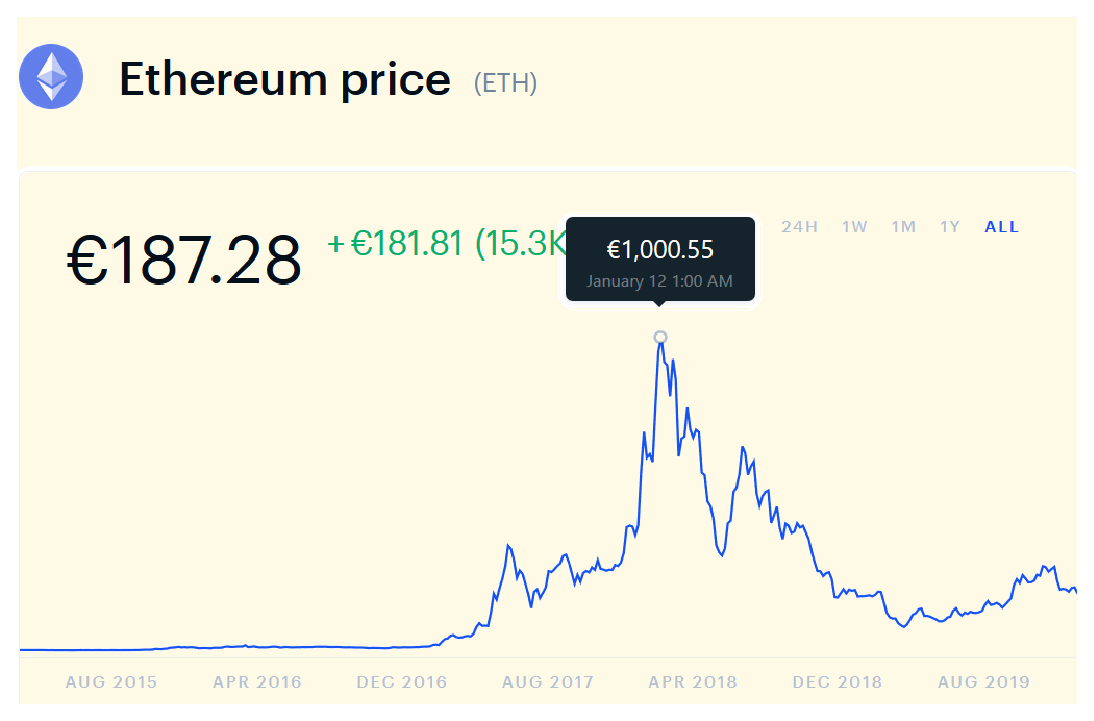
\includegraphics[keepaspectratio, width=0.481125\textwidth]{images/ethcurrentprice-sourcecoinbase.eps}
%% %  \caption{Figura 3. Variación cotización ETH (11/08/2019)}
%% %\end{figure}e
%% \\
%% Figure 7. ETH Price chart (11/08/2019). Source: [Coinbase 19]
%% \\
%% \end{center}


%% \subsection{Añadir forma de pago DAI} \label{ch:dai}
%% DAI es una criptomoneda estable (\textit{stablecoin}) que funciona con ETH y que intenta mantener un valor de 1\$. A diferencia de los billetes de banco centralizados, DAI no está respaldado por dólares estadounidenses en una cuenta bancaria. En cambio, está respaldado por garantías en la plataforma Maker [MakerDAO 19].
%% \subsection{Usar Raspberry Pi 4 Modelo B} \label{ch:rpi4modelb}
%% Anunciado en Junio de 2019 y a la venta. Es un hardware que ofrece mejores prestaciones. Por ejemplo, el procesador es un Broadcom BCM2711. Un ARM Cortex-A72 de cuatro núcleos y a 1,5 GHz. Hasta tres veces más eficiente (\textit{benchmark}) que el modelo anterior (Raspberry Pi 3 Modelo B+). También da la posibilidad de elegir entre 1, 2 y 4 GB de RAM.
%% \subsection{Usar Docker Swarm} \label{ch:dockerswarm}
%% Se podría presentar una aplicación descentralizada basada en microservicios. Por ejemplo en microservicios, un contenedor Docker (como en la sección 4) podría verse como un servicio. Entre las ventajas que aporta microservicios estarían:
%% \begin{itemize}
%%  \item Pequeños
%%  \item Independientes
%%  \item Despliegue sencillo
%%  \item Reutilizables
%%  \item Externalización
%%  \item Escalabilidad
%%  \newline
%% \end{itemize}
%% Para ello, Docker ofrece un orquestador (de código abierto) llamado Docker Swarm (véase figura 4). Un nodo \textit{worker} sería nuestra Raspberry Pi y un nodo \textit{manager} sería un centro de control.
%% \begin{center}
%% %\begin{figure}[h]
%% %  \centering
%%   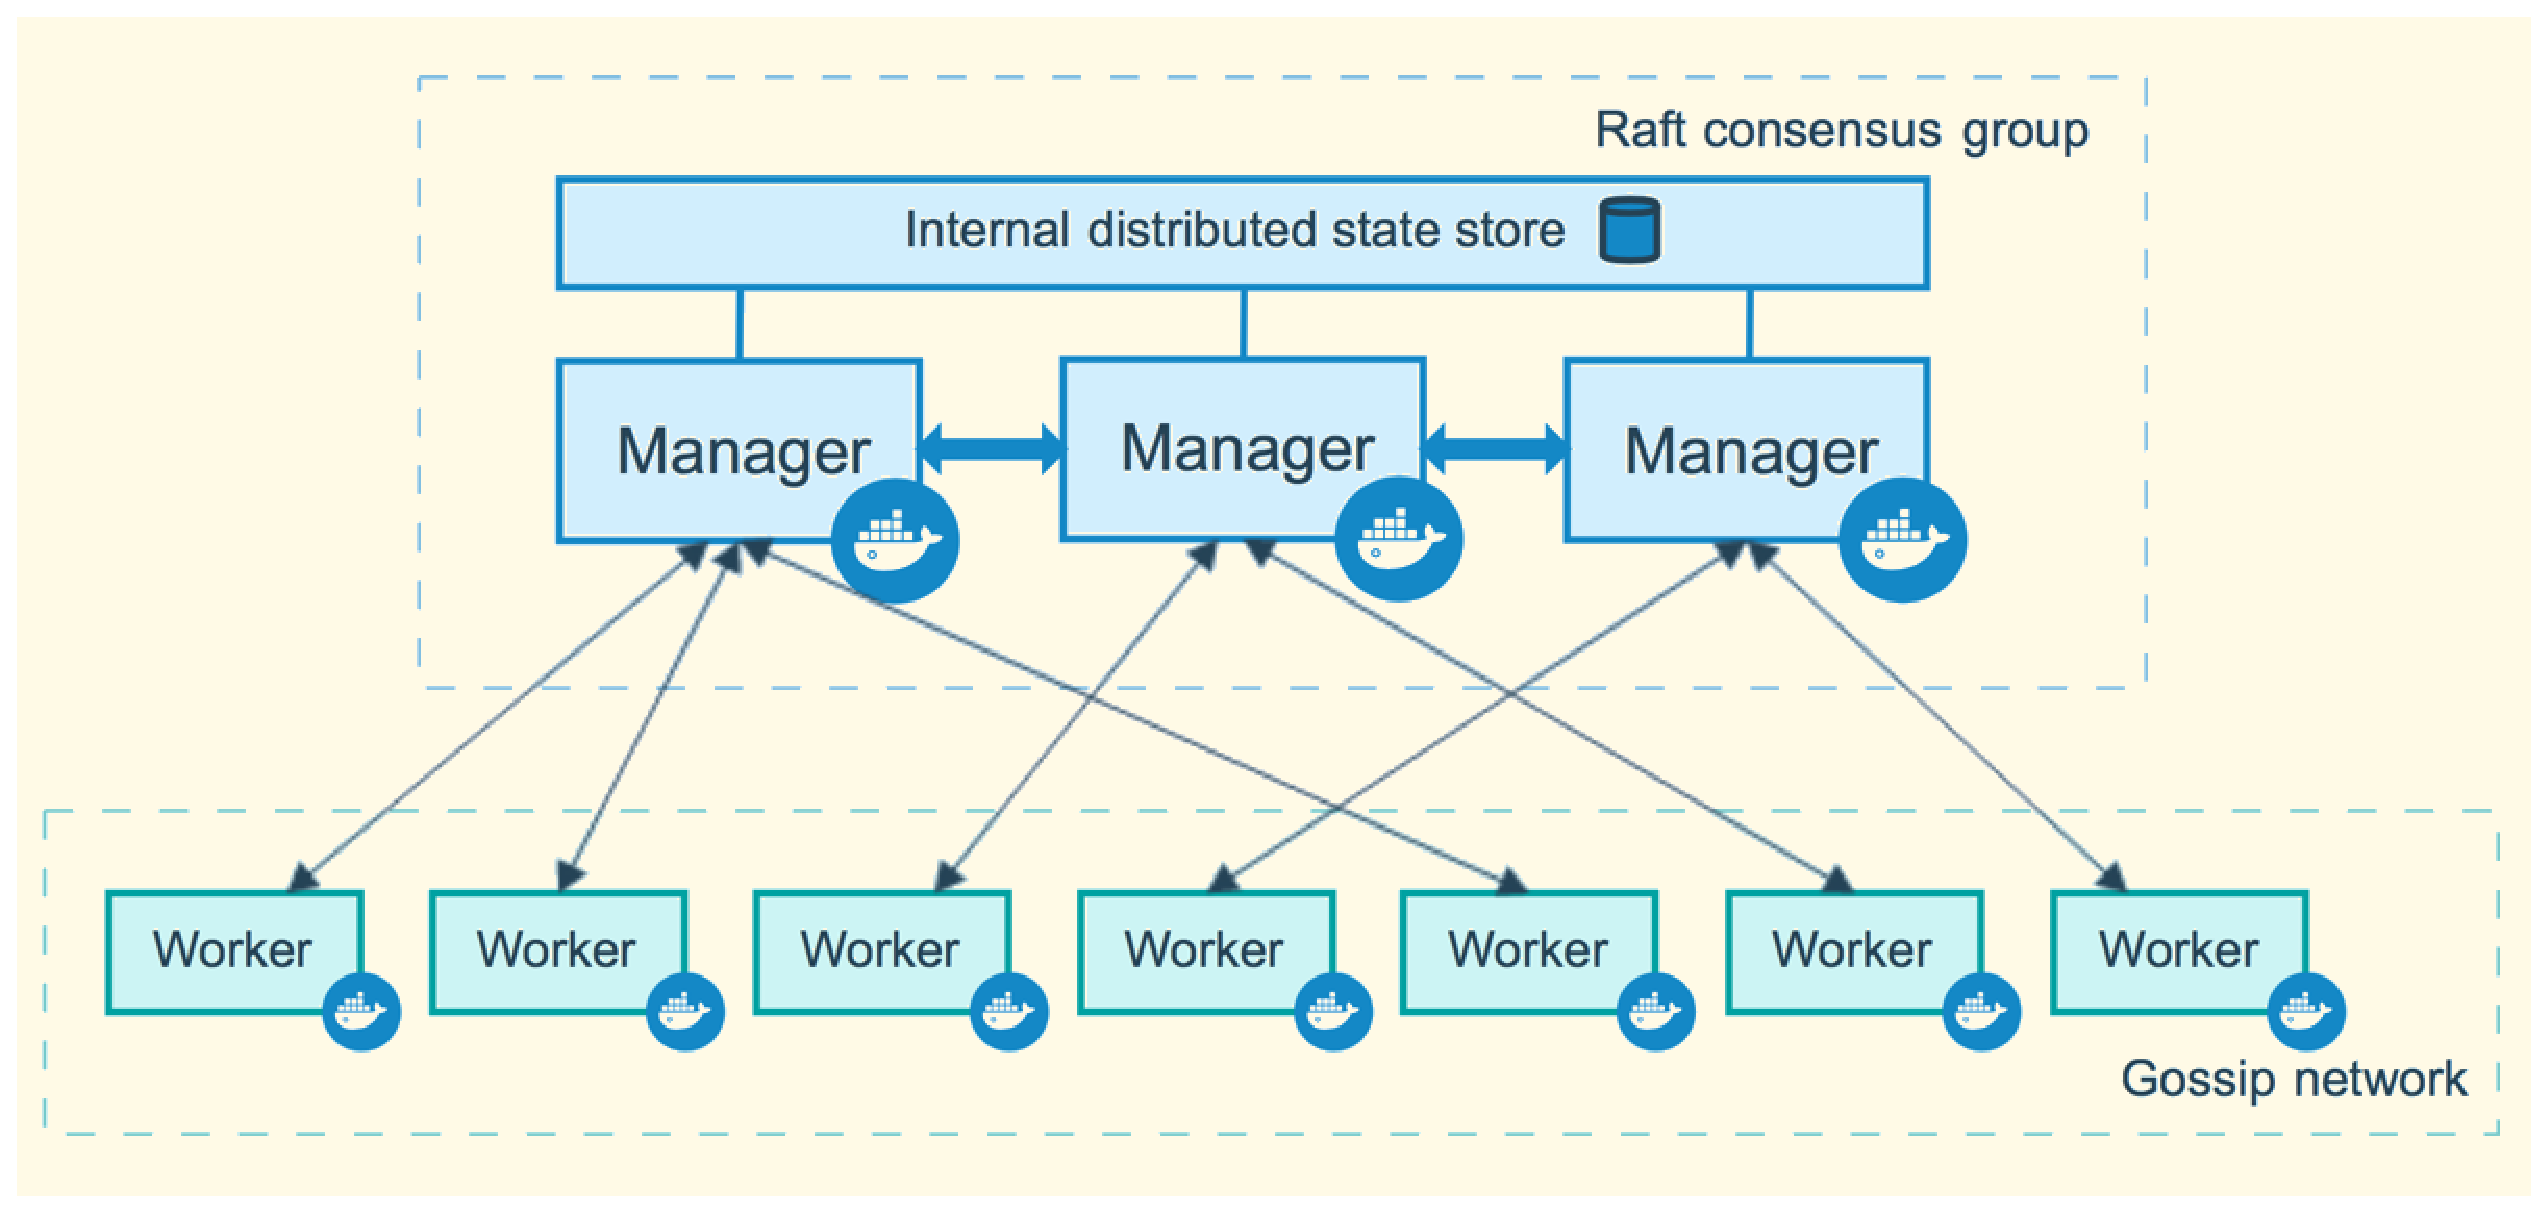
\includegraphics[keepaspectratio, width=0.481125\textwidth]{images/swarm-diagram-sourcedocker.eps}
%% %  \caption{Figura 3. Variación cotización ETH (11/08/2019)}
%% %\end{figure}
%% \\
%% Figura 4. Diagrama Docker Swarm. Fuente: [Docker 19]
%% \\
%% \end{center}

%% \section{Repositorio}\label{sec:repository}
%% El código fuente generado en el proyecto está publicado en un repositorio público de GitHub bajo licencia MIT.
%% \newline\newline
%% \url{https://github.com/ethereum-internet-access}
%% \newline
\begin{thebibliography}{9}

\bibitem{spectrumnh}
  \href{https://uk5g.org/media/uploads/resource_files/Spectrum\_NH\_discussion\_paper\_20Feb19.pdf}{5G Spectrum and Neutral Hosting}, Discussion paper,
  DCMS Phase 1 5G Testbeds \& Trials Program. February 2019.
\bibitem{5g} \href{https://en.wikipedia.org/wiki/5G}{https://en.wikipedia.org/wiki/5G}
\bibitem{sdns} Ian F. Akyildiz and Shih-Chun Lin and Pu Wang.
  \textit{Wireless software-defined networks (W-SDNs) and network function virtualization (NFV) for 5G cellular systems:
    An overview and qualitative evaluation}. Computer Networks, 93, 2015
\bibitem{nfv} J. Ordonez-Lucena, P. Ameigeiras, D. Lopez, J. J. Ramos-Munoz, J. Lorca and J. Folgueira.
  \textit{Network Slicing for 5G with SDN/NFV: Concepts, Architectures, and Challenges}.
   IEEE Communications Magazine, volume 55, issue 5, May 2017.
\bibitem{fon} \href{https://es.wikipedia.org/wiki/La_Fonera}{https://es.wikipedia.org/wiki/La\_Fonera}
\bibitem{hotspotme} \href{https://devpost.com/software/hotspot-me}{https://devpost.com/software/hotspot-me}
\bibitem{hostapd} \href{https://w1.fi/hostapd/}{https://w1.fi/hostapd/}
\bibitem{iptables} \href{https://linux.die.net/man/8/iptables}{https://linux.die.net/man/8/iptables}
\bibitem{dnsmasq} \href{https://en.wikipedia.org/wiki/Dnsmasq}{https://en.wikipedia.org/wiki/Dnsmasq}
\bibitem{osmc} \href{https://osmc.tv/}{https://osmc.tv/}

\bibitem{state-channel-contract-a}
  \href{https://github.com/ethereum-internet-access/state-channel-contract-a}{state-channel-contract-a on GitHub}
\bibitem{etherwall}
  \href{https://github.com/ethereum-internet-access/etherwall}{etherwall on GitHub}
\bibitem{infuraProxy}
  \href{https://github.com/ethereum-internet-access/etherwall/blob/master/infuraProxy.js}{infuraProxy on GitHub}

\bibitem{etherdoor}
  \href{https://github.com/ethereum-internet-access/etherdoor}{etherdoor on GitHub}
\bibitem{express}
  \href{https://expressjs.com/}{https://expressjs.com/}

\bibitem{ganache}
  \href{https://github.com/trufflesuite/ganache-cli}{https://github.com/trufflesuite/ganache-cli}

\bibitem{express}
  \href{https://expressjs.com/}{https://expressjs.com/}
\bibitem{mocha}
  \href{https://mochajs.org/}{https://mochajs.org/}
\bibitem{chai}
  \href{https://chaijs.com/}{https://chaijs.com/}

\bibitem{5gcity} \href{https://www.5gcity.eu/}{https://www.5gcity.eu/}
\bibitem{allen}  \href{https://github.com/ChristopherA/self-sovereign-identity/blob/master/ThePathToSelf-SovereignIdentity.md}
  {C. Allen.} The Path to Self-Sovereign Identity. GitHub. 25 April 2016.
\bibitem{identicat}
  \href{https://www.coindesk.com/catalonia-government-to-build-dlt-based-identity-platform-for-citizens}
       {D. Palmer.} Catalonia to Build DLT-Based Identity Platform for Citizens. Coindesk. 9 September 2019.


\bibitem{Coinbase19} Ethereum Price (ETH). Coinbase. \href{https://www.coinbase.com/price/ethereum}{https://www.coinbase.com/price/ethereum}
\bibitem{ConsenSys19} Ethereum Smart Contract Best Practices. Security tools. ConsenSys. 12 August 2019.
\bibitem{Docker19} Docker Documentation. How nodes work. 6 September 2019.  \href{https://docs.docker.com/engine/swarm/how-swarm-mode-works/nodes/}{Docker Swarm}
\bibitem{ETHBerlinZwei19} Hackathon ETH Berlin Zwei. 6 September 2019. \href{https://ethberlinzwei.com/}{https://ethberlinzwei.com/}
\bibitem{Hegedus18} P. Hegedus. \textit{Towards Analyzing the Complexity Landscape of Solidity Based Ethereum Smart Contracts}. 2018 IEEE/ACM 1st International Workshop on Emerging Trends in Software Engineering for Blockchain (WETSEB). 27 May-3 June 2018. \href{https://ieeexplore.ieee.org/document/8445056}{https://ieeexplore.ieee.org/document/8445056}
\bibitem{MakerDAO19} MakerDAO. Stability for the blockchain.  \href{https://makerdao.com/en/dai}{https://makerdao.com/en/dai}
\bibitem{Munoz18} J. L. Muñoz. Docker Containers. Notes from masterclasses. Master’s degree in Blockchain Technologies. 1st Edition. UPC School. 29 November 2018.
\bibitem{Nakamoto08} S. Nakamoto. \textit{Bitcoin: A Peer-to-Peer Electronic Cash System}. 31 October 2008.  \href{https://bitcoin.org/bitcoin.pdf}{https://bitcoin.org/bitcoin.pdf}
\bibitem{RaspberryPi19} Raspberry Pi 3 Modelo B - Placa Base (1.2 GHz Quad-Core Arm Cortex-A53, 1 GB RAM, USB 2.0). Amazon. 11 August 2019.
\bibitem{RaspberryPiBuy19} Raspberry Pi FAQs. BUYING AND SHIPPING. Where can I buy a Raspberry Pi?. Official Web Page. 11 August 2019.  (\href{https://www.raspberrypi.org/help/faqs/#buyingWhere}{Link})
\bibitem{Stallings04} W. Stallings. \textit{Comunicaciones y redes de computadores}. 1 September 2004. 904 pages. Pearson Prentice Hall. ISBN-13: 978-8420541105.



\bibitem{berec16} Report on OTT services. BEREC (Body of European Regulators for Electronic Communications). January 2016.
\bibitem{eecc18} Directive (EU) 2018/1972 of the European
  Parliament and of the Council of 11 December 2018 establishing the
  European Electronic Communications Code (Recast)Text with EEA
  relevance. PE/52/2018/REV/1.

\bibitem{gdpr16} Regulation (EU) 2016/679 of the European
  Parliament and of the Council of 27 April 2016 on the protection of
  natural persons with regard to the processing of personal data and
  on the free movement of such data, and repealing Directive 95/46/EC
  (General Data Protection Regulation) (Text with EEA relevance).

\bibitem{h202018} Ethics and data protection. European
  Commission (DG Research and Innovation). 14 November 2018.

\bibitem{tata17} A Systematic Approach to Ensuring GDPR
    Compliance: Key Action Items for Telecom Operators. White
    Paper. Tata Consultancy Services. 2017.

\bibitem{neutral} Enabling Neutral Host
Network Economics: CCS case study, GSM Association. August 2018.
\end{thebibliography}
\clearpage


\end{multicols}


\end{document}
